%%%%%%%%%%%%%%%%%%%%%%%%%%%%%%%%%%%%%%%%%%%%%%%%%%%%%%%%%%%%
%%  This Beamer template was created by Cameron Bracken.
%%  Anyone can freely use or modify it for any purpose
%%  without attribution.
%%
%%  Last Modified: January 9, 2009
%%

\documentclass[xcolor=x11names,compress,8pt]{beamer}
%\usetheme{AnnArbor}
%\usetheme{Boadilla}
%\usetheme{Madrid}
%% General document %%%%%%%%%%%%%%%%%%%%%%%%%%%%%%%%%%
\usepackage{graphicx} 	% to include figures
\usepackage{tikz}
\usepackage{amsmath}		% for math AMS fonts
\usepackage{subfigure}	% to have figures in figures
\usepackage{multimedia}	% to include movies
\usepackage{hyperref}	% for hyper reference
\usepackage{animate}		% for animation
%\hypersetup{pdfpagemode=FullScreen}	% start pdf in presentation mode
\usetikzlibrary{decorations.fractals}
\usepackage{lscape}						% allow to get landscape style for single page
\usepackage{seqsplit}
\usepackage{fancybox}
\usepackage{framed,color}
\usepackage{xcolor}
%\usepackage[usenames,dvipsnames]{xcolor}			% allows to coustomize color
\definecolor{darkred}{rgb}{0.7,0.0,0.0}			% 70% of red color
\definecolor{darkgreen}{rgb}{0.0,0.65,0.0}		% 70% of green color
\definecolor{darkblue}{rgb}{0.0,0.0,0.7}			% 70% of blue color
\definecolor{light-red}{rgb}{1.0,0.85,0.85}		% define light-red color
\definecolor{light-green}{rgb}{0.85,1.0,0.85}	% define light-green color
\definecolor{light-blue}{rgb}{0.83,0.85,1.0}		% define light-blue color
\definecolor{light-gray}{gray}{0.88}				% define light-gray color

%\usepackage{mathastext} 						% no italic font
%\usepackage[LGRgreek]{mathastext}

\usepackage[framemethod=tikz]{mdframed}
\usepackage{tcolorbox}
\usepackage{lipsum}

\usefonttheme{professionalfonts}
\usepackage{times}
\usepackage{verbatim}
\usetikzlibrary{arrows,shapes}
\usetikzlibrary{patterns}


%%%%%%%%%%%%%%%%%%%%%%%%%%%%%%%%%%%%%%%%%%%%%%%%%%%%%%


%% Beamer Layout %%%%%%%%%%%%%%%%%%%%%%%%%%%%%%%%%%
\useoutertheme[subsection=false,shadow]{miniframes}
\useinnertheme{default}
\usefonttheme{serif}
%\usepackage{palatino}
\usepackage{lmodern}

\setbeamerfont{title like}{shape=\scshape}
\setbeamerfont{frametitle}{shape=\scshape}

%\setbeamercolor*{lower separation line head}{bg=DeepSkyBlue4}
\setbeamercolor*{lower separation line head}{bg=darkblue}
\setbeamercolor*{normal text}{fg=black,bg=white} 
\setbeamercolor*{alerted text}{fg=red} 
\setbeamercolor*{example text}{fg=black} 
\setbeamercolor*{structure}{fg=black} 
\setbeamercolor*{link text}{fg=blue} 

\setbeamercolor*{palette tertiary}{fg=black,bg=black!10}  
\setbeamercolor*{palette quaternary}{fg=black,bg=black!10} 

\setbeamercovered{transparent}		% transparent overlays

%\setbeamercolor{footnote mark}{fg=red}

\renewcommand{\(}{\begin{columns}}
\renewcommand{\)}{\end{columns}}
\newcommand{\<}[1]{\begin{column}{#1}}
\renewcommand{\>}{\end{column}}

%% Don't draw action buttons in the slides.
\setbeamertemplate{navigation symbols}{}%remove navigation symbols
%% Don't count backup slides in the main content (fix the total no of pages)
\usepackage{appendixnumberbeamer}

%%%%%%%%%%%%%%%%%%%%%%%%%%%%%%%%%%%%%%%%%%%%%%%%%%

%\fontsize{6pt}{7.2}\selectfont
%\newcommand\Fontvi{\fontsize{6}{7.2}\selectfont}

\def\shorttitle{Q-weak}

\def\vanue{DNP 2013}

\setbeamertemplate{footline}{%
\begin{beamercolorbox}{section in head/foot}
%    \color{gray}\vskip2pt~ \insertsection\hfill\insertpagenumber{} of \insertpresentationendpage{} ~\vskip2pt
    \color{black}\vskip2pt~ Nuruzzaman [HU]\hfill \vanue \hfill \shorttitle \hfill \insertpagenumber{} \color{gray} of \insertpresentationendpage{} %~\vskip2pt
\end{beamercolorbox}
}
%\let\oldfootnotesize\footnotesize
%\renewcommand*{\footnotesize}{\oldfootnotesize\large}


\def\logos{
%\vspace{\fill}
\begin{figure}[!b]
\begin{minipage}{8.5cm}
  
\includegraphics[width=2.6cm]{figures/HamptonUniversityLogo}
\end{minipage}%
\begin{minipage}{8.5cm}
  
\includegraphics[width=2.6cm]{figures/jlab_logo}
\end{minipage}
\end{figure}
}

%%%%%%%%%%%%%%%%%%%%%%%%%%%%%%%%%%%%%%%%%%%%%%%%%%%%%%
%%%%%%%%%%%%%%%%%%%%%%%%%%%%%%%%%%%%%%%%%%%%%%%%%%%%%%



\begin{document}

%%%%%%%%%%%%%%%%%%%%%%%%%%%%%%%%%%%%%%%%%%%%%%%%%%%%%%
%%%%%%%%%%%%%%%%%%%%%%%%%%%%%%%%%%%%%%%%%%%%%%%%%%%%%%
\section{\scshape Introduction}
\begin{frame}[plain]

\title{

\begin{center}
\begin{tcolorbox}[colback=darkblue,colframe=darkblue]
\fontsize{16pt}{7.2}\selectfont
\begin{center}
%\textbf{
\color{white}{Beam Normal Single Spin Asymmetry in the N-to-$\Delta$ Transition}
%}
\end{center}
\end{tcolorbox}
\end{center}
}

\author{
	Nuruzzaman\\
	\fontsize{6pt}{7.2}\selectfont	
	(\url{https://userweb.jlab.org/~nur/})\\
	\vspace{0.25cm}
	\fontsize{8pt}{7.2}\selectfont	
	for the Q-weak Collaboration\\
}
\date{
	\vspace{0.5cm}
	
	2013 Fall Meeting of the APS Division of Nuclear Physics\\
	Newport News, VA

	\vspace{0.5cm}
		
	\fontsize{8pt}{7.2}\selectfont
	\color{darkgreen}{
%	\today
	26th October 2013
	}
	\logos
}
\titlepage
\setcounter{framenumber}{0}
\newcounter{slidenumber}
\setcounter{slidenumber}{\insertpagenumber}
\end{frame}

%%%%%%%%%%%%%%%%%%%%%%%%%%%%%%%%%%%%%%%%%%%%%%%%%%%%%%
%%%%%%%%%%%%%%%%%%%%%%%%%%%%%%%%%%%%%%%%%%%%%%%%%%%%%%
\AtBeginSection[]
{
  \begin{frame}%[noframenumbering]
  \frametitle{Overview}
  \tableofcontents[currentsection]
  \addtocounter{framenumber}{-1}
%  \addtocounter{framenumber}{-1}
\addtocounter{slidenumber}{-\insertframestartpage}%
  \end{frame}
}

%%%%%%%%%%%%%%%%%%%%%%%%%%%%%%%%%%%%%%%%%%%%%%%%%%%%%%
%%%%%%%%%%%%%%%%%%%%%%%%%%%%%%%%%%%%%%%%%%%%%%%%%%%%%%
\section{\scshape Basics}
\begin{frame}

\begin{equation} \label{equ:eqPhysicsAsymmetry101}
\textcolor{black}{B_{\rm n}} = \textcolor{magenta}{M_{\rm kin}} \left[ \frac{\frac{\textcolor{red}{\epsilon_{\rm reg}}}{\textcolor{darkgreen}{P}} - \displaystyle\sum_{i=1}^{4} \textcolor{blue}{B_{\rm bi}f_{\rm bi}} }{1 - \displaystyle\sum_{i=1}^{4}\textcolor{blue}{f_{\rm bi}}} \right] 
\end{equation}

\begin{equation} \label{equ:eqPhysicsAsymmetry101}
\textcolor{black}{B_{n}} = \textcolor{magenta}{M_{total}} \left[ \frac{\frac{\textcolor{red}{\epsilon_{reg}}}{\textcolor{darkgreen}{P}} - \displaystyle\sum_{i=1}^{4} \textcolor{blue}{B_{bi}f_{bi}} }{1 - \displaystyle\sum_{i=1}^{4}\textcolor{blue}{f_{bi}}} \right] 
\end{equation}

\begin{equation} \label{equ:eqPhysicsAsymmetry102}
\textcolor{red}{\epsilon_{reg} = \epsilon_{raw} - \displaystyle\sum_{i=1}^{5} \left(\frac{\partial \epsilon_{raw}}{\partial T_{i}}\right)\Delta T_{i}  }
\end{equation}

\begin{equation} \label{equ:eqPhysicsAsymmetry103}
\textcolor{magenta}{M_{total} = M_{RC}M_{Det}M_{Q^{2}}M_{\phi}}
\end{equation}

\begin{equation} \label{equ:eqPhysicsAsymmetry104}
\textcolor{black}{B_{\rm n}} = \textcolor{magenta}{M_{\rm RC}M_{\rm Det}M_{\rm Q^{2}}M_{\rm\phi}} \left[ \frac{\frac{\textcolor{red}{\epsilon_{\rm reg}}}{\textcolor{darkgreen}{P}} - \textcolor{blue}{ B_{\rm Al}f_{\rm Al} - B_{\rm BB}f_{\rm BB} - B_{\rm QTor}f_{\rm QTor} - B_{\rm el}f_{\rm el} } }{1 - \textcolor{blue}{ f_{\rm Al} - f_{\rm BB} - f_{\rm QTor} - f_{\rm el} }} \right] 
\end{equation}


\end{frame}




%%%%%%%%%%%%%%%%%%%%%%%%%%%%
\begin{frame}

\begin{equation} \label{equ:eqPhysicsAsymmetry104}
\textcolor{black}{B_{\rm n}} =  \textcolor{magenta}{M_{\rm kin}} \left[ \frac{\frac{\textcolor{red}{\epsilon_{\rm reg}}}{\textcolor{darkgreen}{P}} - \textcolor{blue}{ B_{\rm Al}f_{\rm Al} - B_{\rm BB}f_{\rm BB} - B_{\rm QTor}f_{\rm QTor} - B_{\rm el}f_{\rm el} } }{1 - \textcolor{blue}{ f_{\rm Al} - f_{\rm BB} - f_{\rm QTor} - f_{\rm el} }} \right] 
\end{equation}

\begin{equation} \label{equ:eqPhysicsAsymmetry104}
\frac{\textcolor{red}{\epsilon_{reg}}}{\textcolor{darkgreen}{P}} = \frac{(1 - \textcolor{blue}{f_{total}})}{\textcolor{magenta}{M_{kin}}}B_{n} + \textcolor{blue}{B_{el}f_{el}} + \textcolor{blue}{others}
\end{equation}

\begin{equation} \label{equ:eqPhysicsAsymmetry104}
\frac{(1 - \textcolor{blue}{f_{total}})}{\textcolor{magenta}{M_{kin}}}B_{n} = \frac{\textcolor{red}{\epsilon_{reg}}}{\textcolor{darkgreen}{P}} - \textcolor{blue}{B_{el}f_{el}} - \textcolor{blue}{others}
\end{equation}


\begin{equation} \label{equ:eqPhysicsAsymmetry104}
\textcolor{black}{B_{n}} =  \frac{\frac{\textcolor{red}{\epsilon_{reg}}}{\textcolor{green}{P}} - \textcolor{blue}{ B_{Al}f_{Al} - B_{BB}f_{BB} - B_{QTor}f_{QTor} - B_{el}f_{el} } }{1 - \textcolor{blue}{ f_{Al} - f_{BB} - f_{QTor} - f_{el} }}
\end{equation}

\begin{itemize}
\item 
$\textcolor{red}{\epsilon_{reg}} = \epsilon_{reg}^{in}M_{\phi}$, $\epsilon_{reg}^{in}$ is the measured asymmetry

\item 
$\textcolor{blue}{B_{Al}} = \epsilon_{reg}^{Al}M_{\phi}/P$, 
$\epsilon_{reg}^{Al} = (\epsilon_{reg}^{DS-Al} + \epsilon_{reg}^{US-Al})/2$
\item 
$\textcolor{blue}{f_{Al}}$, measured

\item 
$\textcolor{blue}{B_{BB}}$ = 0 $\pm$ 0.313~ppm, AncELOG 122
\item 
$\textcolor{blue}{f_{BB}}$, measured

\item 
$\textcolor{blue}{B_{Qtor}}$ = 0 $\pm$ 10~ppm
\item 
$\textcolor{blue}{f_{QTor}}$, measured

\item 
$\textcolor{blue}{B_{el}}$ = $\sqrt{\frac{Q_{in}^{2}}{Q_{el}^{2}}}B_{T}^{el}$, $B_{T}^{el}$ is Buddhini's final asymmetry. Will change after calculation from Gorchtein. Mark D. has preliminary no. but not finalized yet. 
\item 
$\textcolor{blue}{f_{el}}$, simulation


\end{itemize}

\end{frame}

%%%%%%%%%%%%%%%%%%%%%%%%%%%%
\begin{frame}

\begin{equation} \label{equ:eqPhysicsAsymmetry104}
\textcolor{black}{B_{n}} = \textcolor{magenta}{M_{RC}M_{Det}M_{Q^{2}} } \left[ \frac{\frac{\textcolor{red}{\epsilon_{reg}}}{\textcolor{green}{P}} - \textcolor{blue}{ B_{Al}f_{Al} - B_{BB}f_{BB} - B_{QTor}f_{QTor} - B_{el}f_{el} } }{1 - \textcolor{blue}{ f_{Al} - f_{BB} - f_{QTor} - f_{el} }} \right] 
\end{equation}

\begin{itemize}
\item 
$\textcolor{red}{\epsilon_{reg}} = \epsilon_{reg}^{in}M_{\phi}$, $\epsilon_{reg}^{in}$ is the measured asymmetry

\item 
$\textcolor{blue}{B_{Al}} = \epsilon_{reg}^{Al}M_{\phi}/P$, 
$\epsilon_{reg}^{Al} = (\epsilon_{reg}^{DS-Al} + \epsilon_{reg}^{US-Al})/2$
\item 
$\textcolor{blue}{f_{Al}}$, measured

\item 
$\textcolor{blue}{B_{BB}}$ = 0
\item 
$\textcolor{blue}{f_{BB}}$, measured

\item 
$\textcolor{blue}{B_{Qtor}}$ = 0
\item 
$\textcolor{blue}{f_{QTor}}$, measured

\item 
$\textcolor{blue}{B_{el}}$ = $\sqrt{\frac{Q_{in}^{2}}{Q_{el}^{2}}}B_{T}^{el}$, $B_{T}^{el}$ is Buddhini's final asymmetry. Will change after calculation from Gorchtein
\item 
$\textcolor{blue}{f_{el}}$, simulation

\item 
$\textcolor{magenta}{M_{RC}}$, needs update

\item 
$\textcolor{magenta}{M_{Det}}$, needs update

\item 
$\textcolor{magenta}{M_{Q^{2}}}$?, probably we should change it to $M_{\theta}$ as we will be quoting numbers at $\theta$ = 8.3 degrees. But need to know the uncertainty on $\theta$. 

\end{itemize}




\end{frame}
%%%%%%%%%%%%%%%%%%%%%%%%%%%%
%\begin{frame}
%
%\end{frame}

\subsection{\scshape Q-weak First Result}
\begin{frame}


\begin{equation} \label{equ:eqPhysicsAsymmetry211}
\textcolor{black}{A_{\rm ep}} = \textcolor{magenta}{R_{\rm total}} \left[ \frac{\displaystyle\frac{\textcolor{red}{A_{\rm msr}}}{\textcolor{darkgreen}{P}} - \displaystyle\sum_{i=1}^{4} \textcolor{blue}{A_{\rm bi}f_{\rm bi}} }{1 - \displaystyle\sum_{i=1}^{4}\textcolor{blue}{f_{\rm bi}}} \right] 
\end{equation}


\begin{equation} \label{equ:eqPhysicsAsymmetry211}
\textcolor{red}{A_{\rm msr} = A_{\rm raw} + A_{T} + A_{L} + A_{\rm reg} }
\end{equation}

\begin{equation} \label{equ:eqPhysicsAsymmetry211}
\textcolor{magenta}{R_{\rm total} = R_{\rm RC}R_{\rm Det}R_{\rm Bin}R_{Q^{2}} }
\end{equation}


\begin{equation} \label{equ:eqPhysicsAsymmetry211}
\textcolor{black}{A_{\rm ep}} = \textcolor{magenta}{R_{\rm RC}R_{\rm Det}R_{\rm Bin}R_{\rm Q^{2}}} \left[ \frac{\displaystyle\frac{\textcolor{red}{A_{\rm msr}}}{\textcolor{darkgreen}{P}} - \textcolor{blue}{A_{\rm Al}f_{\rm Al}} - \textcolor{blue}{A_{\rm BB}f_{\rm BB}} - \textcolor{blue}{A_{\rm QTor}f_{\rm QTor}} - \textcolor{blue}{A_{\rm in}f_{\rm in}} }{1 - \textcolor{blue}{f_{\rm Al}} - \textcolor{blue}{f_{\rm BB}} - \textcolor{blue}{f_{\rm QTor}} - \textcolor{blue}{f_{\rm el}} } \right] 
\end{equation}

\end{frame}


\subsection{Q-weak First Result 2}
\begin{frame}{Q-weak First Result 2}


\begin{table}[th]
\centering
\begin{tabular}{@{} l @{}|@{} c @{} c  r }
\hline
 & Correction & \multicolumn{2}{c}{Contribution} \\
  & Value [ppb] & \multicolumn{2}{c}{to $\Delta A_{\rm ep}$ [ppb]} \\ 
  \hline 
%  \hdashrule
%  \hdashline
%  \dottedline
%\dashline
%\hline[dashed]
  \multicolumn{4}{c}{Normalization Factors Applied to \textcolor{red}{$A_{\rm raw}$} } \\ 
  \hline 
Beam Polarization 1/\textcolor{darkgreen}{P} & -21 & \multicolumn{2}{r}{5} \\
Kinematics \textcolor{magenta}{$R_{\rm total}$} & 5 & \multicolumn{2}{r}{9} \\ 
Background Dilution 1/(1-\textcolor{blue}{$f_{\rm total}$}) & -7 & \multicolumn{2}{r}{-} \\ 
\hline
\multicolumn{4}{c}{Asymmetry Corrections} \\
\hline  
Beam Asymmetries \textcolor{red}{$\kappa A_{\rm reg}$} & -40 & \multicolumn{2}{r}{13} \\ 
Transverse Polarization \textcolor{red}{$\kappa A_{T}$} & 0 & \multicolumn{2}{r}{5} \\ 
Detector Linearity \textcolor{red}{$\kappa A_{L}$} & 0 & \multicolumn{2}{r}{4} \\ 
\hline
Backgrounds  & \textcolor{blue}{$\kappa Pf_{\rm bi}A_{\rm bi}$} & \textcolor{blue}{$\delta(f_{\rm bi})$} & \textcolor{blue}{$\delta(A_{\rm bi})$} \\ 
\hline 
\hspace{0.1cm} Target windows (\textcolor{blue}{\rm Al}) & -58 & 4 & 8 \\ 
\hspace{0.1cm} Beamline scattering (\textcolor{blue}{\rm BB}) & 11 & 3 & 23 \\ 
\hspace{0.1cm} Other neutral bkg (\textcolor{blue}{\rm QTor}) & 0 & 1 & \textless 1 \\ 
\hspace{0.1cm} Inelastics (\textcolor{blue}{\rm in}) & 1 & 1 & \textless 1 \\ 
\hline

\end{tabular}
\caption{Summary of corrections and the associated systematic uncertainty, in parts per billion. The table shows the contributions of normalization factors on $A_{raw}$, then the properly normalized contributions from other sources. Background correction terms listed here include only $R_{tot} f_{i}A_{i}/(1 - f_{tot})$ uncertainties in $A_{ep}$ due to dilution fraction and background asymmetry uncertainties are noted separately.}
\label{tab-3}       % Give a unique label
%\vspace*{5cm}  % with the correct table height
\end{table}


\end{frame}



\begin{frame}{Beam Normal Single Spin Asymmetry 2}

\begin{table}[!h]
\begin{center}
  \begin{tabular}{ l | c | c | c }
%    \hline
    \noalign{\hrule height 1pt}
    \multicolumn{4}{c}{Input parameters} \\
    \hline    
    Measured regressed asymmetry (\textcolor{red}{$A_{M}^{in}$})	&	\multicolumn{3}{l}{5.127 $\pm$ 0.455~ppm} (Det. acpt. corrected) \\
    Beam polarization		(\textcolor{darkgreen}{P})						&	\multicolumn{3}{l}{0.875 $\pm$ 0.009} \\
    Detector acceptance correction		&	\multicolumn{3}{l}{0.9938} \\
%	  \hline 
    \noalign{\hrule height 1pt}
    \multicolumn{4}{c}{Background corrections} \\
    \hline
    Quantity 		&	Asymmetry & Dilution & Correction \\
    &	(\textcolor{blue}{$A_{bi}$}) & (\textcolor{blue}{$f_{bi}$}) & $c_{i}=\kappa \textcolor{darkgreen}{P}\textcolor{blue}{A_{bi}f_{bi}}$ \\
    & [ppm] &  & [ppm] \\
	\hline
	Target windows (\textcolor{blue}{b1}) 		& 9.185 $\pm$ 1.279 		& 0.033 $\pm$ 0.002 & 1.364 \\
	Beamline scattering (\textcolor{blue}{b2}) 	& 2.239 $\pm$ 6.843 		& 0.018 $\pm$ 0.001 & 0.180 \\
	Other neutral bkg. (\textcolor{blue}{b3}) 	& 0.000 $\pm$ 0.200 		& 0.024 $\pm$ 0.010 & 0.000 \\
	Elastic asymmetry (\textcolor{blue}{b4}) 	& -4.885 $\pm$ 0.093	& 0.701 $\pm$ 0.070 & -13.809 \\
%    \hline 
    \noalign{\hrule height 1pt}
    \multicolumn{4}{c}{Other corrections} \\
    \hline
    Radiative correction (\textcolor{magenta}{$R_{RC}$})		&	\multicolumn{3}{l}{1.010 $\pm$ 0.004} \\
    Detector bias (\textcolor{magenta}{$R_{Det}$})					&	\multicolumn{3}{l}{0.998 $\pm$ 0.001} \\
    $Q^{2}$ acceptance (\textcolor{magenta}{$R_{Q^{2}}$})	&	\multicolumn{3}{l}{1.000 $\pm$ 0.012} \\
%	Azimuthal acceptance (\textcolor{magenta}{$R_{\phi}$})	&	\multicolumn{3}{l}{1.006 $\pm$ 0.004} \\
%	\hline 
    \noalign{\hrule height 1pt}
  	\end{tabular}
  	\caption{Summary of input quantities.}
  \label{tab:PhysicsAsymInput}
\end{center}
\end{table}

\end{frame}

%%%%%%%%%%%%%%%%%%%%%%%%%%%%%%%%%%%%%%%%%%%%%%%%%%%%%%
%%%%%%%%%%%%%%%%%%%%%%%%%%%%%%%%%%%%%%%%%%%%%%%%%%%%%%
\section{\scshape Methodology}
\subsection{Frame 61}

\begin{frame}{Frame 61}

\fontsize{6pt}{7.2}\selectfont

\begin{equation} \label{equ:qweak1}
A_{ep} = \left[ \frac{-G_{F}Q^{2}}{4 \sqrt{2}\pi\alpha} \right] \left[ \frac{\textcolor{blue}{\varepsilon} \textcolor{darkgreen}{G_{E}^{p\gamma}}G_{E}^{pZ} + \textcolor{blue}{\tau} \textcolor{darkgreen}{G_{M}^{p\gamma}}G_{M}^{pZ} - (1-4\sin^{2}\theta_{W})\textcolor{blue}{\varepsilon^{\prime}}\textcolor{darkgreen}{G_{M}^{p\gamma}}\textcolor{red}{G_{A}^{Z}} } { \textcolor{blue}{\varepsilon}(\textcolor{darkgreen}{G_{E}^{p\gamma}})^{2} + \textcolor{blue}{\tau}(\textcolor{darkgreen}{G_{M}^{p\gamma}})^{2} } \right]
\end{equation}

\begin{equation} \label{equ:qweak2}
\textcolor{blue}{\varepsilon} = \frac{1}{1 + 2(1+\textcolor{blue}{\tau})\tan^{2}\frac{\theta}{2}}, \textcolor{blue}{\varepsilon^{\prime}} = \sqrt{\textcolor{blue}{\tau}(1+\textcolor{blue}{\tau})(1 - \textcolor{blue}{\varepsilon}^{2})}, \textcolor{blue}{\tau} = \frac{Q^{2}}{4M}
\end{equation}

\begin{equation} \label{equ:qweak3}
G_{E,M}^{pZ} = (1 - 4\sin^{2} \theta_{W}) \textcolor{darkgreen}{G_{E,M}^{p\gamma}} - \textcolor{darkgreen}{G_{E,M}^{n\gamma}} - \textcolor{purple}{G_{E,M}^{s}}
\end{equation}

\begin{equation} \label{equ:qweak4}
\frac{A_{ep}}{A_{0}} = \left[ \frac{\textcolor{blue}{\varepsilon} \textcolor{darkgreen}{G_{E}^{p\gamma}} (Q_{W}^{p} \textcolor{darkgreen}{G_{E}^{p\gamma}} - \textcolor{darkgreen}{G_{E}^{n\gamma}} - \textcolor{purple}{G_{E}^{s}} ) + \textcolor{blue}{\tau} \textcolor{darkgreen}{G_{M}^{p\gamma}} (Q_{W}^{p} \textcolor{darkgreen}{G_{M}^{p\gamma}} - \textcolor{darkgreen}{G_{M}^{n\gamma}} - \textcolor{purple}{G_{M}^{s}} ) - (1-4\sin^{2}\theta_{W})\textcolor{blue}{\varepsilon^{\prime}}\textcolor{darkgreen}{G_{M}^{p\gamma}}\textcolor{red}{G_{A}^{Z}} } { \textcolor{blue}{\varepsilon}(\textcolor{darkgreen}{G_{E}^{p\gamma}})^{2} + \textcolor{blue}{\tau}(\textcolor{darkgreen}{G_{M}^{p\gamma}})^{2} } \right]
\end{equation}

\begin{equation} \label{equ:qweak5}
\frac{A_{ep}}{A_{0}} = Q_{W}^{p}\left[ \frac{\textcolor{blue}{\varepsilon}(\textcolor{darkgreen}{G_{E}^{p\gamma}})^{2} + \textcolor{blue}{\tau}(\textcolor{darkgreen}{G_{M}^{p\gamma}})^{2} }{ \textcolor{blue}{\varepsilon}(\textcolor{darkgreen}{G_{E}^{p\gamma}})^{2} + \textcolor{blue}{\tau}(\textcolor{darkgreen}{G_{M}^{p\gamma}})^{2} } \right] + \left[(-1)\frac{\textcolor{blue}{\varepsilon}\textcolor{darkgreen}{G_{E}^{p\gamma}}\textcolor{darkgreen}{G_{E}^{n\gamma}} + \textcolor{blue}{\tau}\textcolor{darkgreen}{G_{M}^{p\gamma}}\textcolor{darkgreen}{G_{M}^{n\gamma}} }{ \textcolor{blue}{\varepsilon}(\textcolor{darkgreen}{G_{E}^{p\gamma}})^{2} + \textcolor{blue}{\tau}(\textcolor{darkgreen}{G_{M}^{p\gamma}})^{2} } \right]  + \left[(-1)\frac{(1-4\sin^{2}\theta_{W})\textcolor{blue}{\varepsilon^{\prime}}\textcolor{darkgreen}{G_{M}^{p\gamma}}\textcolor{red}{G_{A}^{Z}} }{ \textcolor{blue}{\varepsilon}(\textcolor{darkgreen}{G_{E}^{p\gamma}})^{2} + \textcolor{blue}{\tau}(\textcolor{darkgreen}{G_{M}^{p\gamma}})^{2} } \right]
\end{equation}

\fontsize{6pt}{7.2}\selectfont

As $\theta$ $\rightarrow$ 0, $\varepsilon$ $\rightarrow$ 1, and $\tau$ $\ll$ 1


\end{frame}

\begin{frame}{Frame 71}

\fontsize{6pt}{7.2}\selectfont

\begin{equation} \label{equ:qweak5}
A_{Q-weak} = \left[ \frac{-G_{F}Q^{2}}{4 \sqrt{2}\pi\alpha} \right] Q_{W}^{p}\left[ \frac{\textcolor{blue}{\varepsilon}(\textcolor{darkgreen}{G_{E}^{p\gamma}})^{2} + \textcolor{blue}{\tau}(\textcolor{darkgreen}{G_{M}^{p\gamma}})^{2} }{ \textcolor{blue}{\varepsilon}(\textcolor{darkgreen}{G_{E}^{p\gamma}})^{2} + \textcolor{blue}{\tau}(\textcolor{darkgreen}{G_{M}^{p\gamma}})^{2} } \right] = 
\end{equation}

\begin{equation} \label{equ:qweak5}
A_{hadronic} = \left[ \frac{-G_{F}Q^{2}}{4 \sqrt{2}\pi\alpha} \right] Q_{W}^{n}\left[\frac{\textcolor{blue}{\varepsilon}\textcolor{darkgreen}{G_{E}^{p\gamma}}\textcolor{darkgreen}{G_{E}^{n\gamma}} + \textcolor{blue}{\tau}\textcolor{darkgreen}{G_{M}^{p\gamma}}\textcolor{darkgreen}{G_{M}^{n\gamma}} }{ \textcolor{blue}{\varepsilon}(\textcolor{darkgreen}{G_{E}^{p\gamma}})^{2} + \textcolor{blue}{\tau}(\textcolor{darkgreen}{G_{M}^{p\gamma}})^{2} } \right] = 
\end{equation}

\begin{equation} \label{equ:qweak5}
A_{axial} = \left[ \frac{-G_{F}Q^{2}}{4 \sqrt{2}\pi\alpha} \right] G_{A}^{e}\left[\frac{(1-4\sin^{2}\theta_{W})\textcolor{blue}{\varepsilon^{\prime}}\textcolor{darkgreen}{G_{M}^{p\gamma}}\textcolor{red}{G_{A}^{Z}} }{ \textcolor{blue}{\varepsilon}(\textcolor{darkgreen}{G_{E}^{p\gamma}})^{2} + \textcolor{blue}{\tau}(\textcolor{darkgreen}{G_{M}^{p\gamma}})^{2} } \right] = 
\end{equation}

\begin{equation} \label{equ:qweak51}
A_{ep} = A_{Q-weak}  + A_{hadronic}  + A_{axial} = 
\end{equation}

\begin{equation} \label{equ:qweak51}
Q_{W}^{p} = (1-4\sin^{2}\theta_{W}) 
\end{equation}

\begin{equation} \label{equ:qweak51}
\frac{A_{ep}}{A_{0}} = \left[ Q_{W}^{p} + Q^{2} B(Q^{2}, \theta) \right]
\end{equation}

\begin{equation} \label{equ:qweak3}
A_{ep} = \left[ \frac{-G_{F}Q^{2}}{4 \sqrt{2}\pi\alpha} \right] \left[ Q_{W}^{p} + B(Q^{2}, \theta) \right] = A_{0} \left[ Q_{W}^{p} + B(Q^{2}, \theta) \right]
\end{equation}

\begin{equation} \label{equ:qweak5}
A_{ep} = \left[ \frac{-G_{F}Q^{2}}{4 \sqrt{2}\pi\alpha} \right] \left[ Q_{W}^{p} + Q^{2}B(Q^{2}, \theta) \right] = A_{0} \left[ Q_{W}^{p} + Q^{2}B(Q^{2}, \theta) \right]
\end{equation}

\begin{equation} \label{equ:qweak4}
\begin{split}
A_{ep} = A_{0} \left[ Q_{W}^{p} + B(Q^{2}, \theta) \right]\\
A_{0} = \frac{-G_{F}Q^{2}}{4 \sqrt{2}\pi\alpha}
\end{split}
\end{equation}


\begin{equation} \label{equ:qweak6}
\begin{split}
\sigma \approx \vert M_{EM} + M_{weak} \vert^{2} \\
\sigma \approx \vert M_{EM} \vert^{2} + 2M_{EM}^{*}M_{weak} + \vert M_{weak} \vert^{2}  \\
\sigma \approx \vert M_{EM} \vert^{2} 
\end{split}
\end{equation}

\end{frame}
%%%%%%%%%%%%%%%%%%%%%%%%%%%%%%%%%%%%%%%%%%%%%%%%%%%%%%
%%%%%%%%%%%%%%%%%%%%%%%%%%%%%%%%%%%%%%%%%%%%%%%%%%%%%%



\subsection{Beam Normal Single Spin Asymmetry}
\begin{frame}{Beam Normal Single Spin Asymmetry (BNSSA)}


  \begin{columns}[T]
    \begin{column}{0.6\textwidth}
     \begin{block}{}
	% Text here
	\pause
	Measured asymmetry
\begin{equation*} \label{equ:eqdTransverse1}
A_{M} = \frac{\sigma^{\uparrow} - \sigma^{\downarrow}}{\sigma^{\uparrow} + \sigma^{\downarrow}} = - B_{n} \vec{P_{T}} \cdot  \hat{n} = - B_{n}P_{T} \sin(\phi_{det} - \phi_{s})
\end{equation*}

where $\hat{n} = \frac{\vec{k}\times\vec{k^{\prime}} }{\vert \vec{k}\times\vec{k^{\prime}\vert}}$ and $\vec{P_{T}}$ is transverse polarization and $B_{n}$ is BNSSA.

\begin{itemize}
\item Measured asymmetry has a small azimuthal dependence.
\end{itemize}

    \end{block}
    \end{column}
    
    
    \begin{column}{0.4\textwidth}
    \begin{block}{}
	% Image included here
	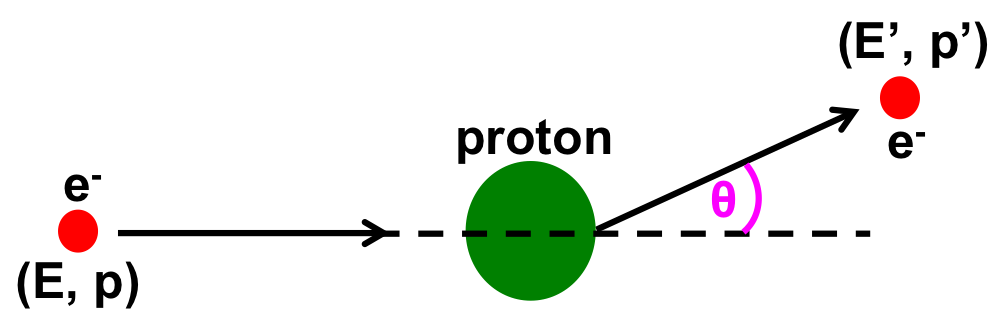
\includegraphics[width=4.0cm]{figures/e-p_scattering}
	\pause
	\\
	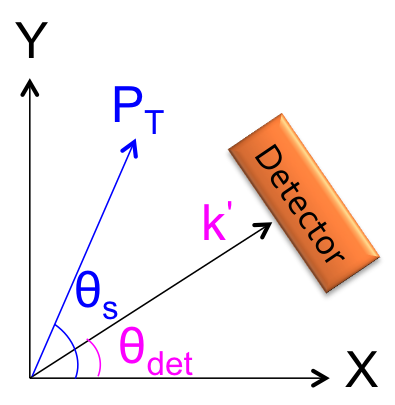
\includegraphics[width=4.0cm]{figures/transverse_diagram}	
    \end{block}
    \end{column}
  \end{columns}

	\pause
Some text some text some text some text some text some text some text some text some text some text some text some text some text some text some text some text some text some text some text some text some text


\end{frame}

%%%%%%%%%%%%%%%%%%%%%%%%%%%%%%%%%%%%%%%%%%%%%%%%%%%%%%
%%%%%%%%%%%%%%%%%%%%%%%%%%%%%%%%%%%%%%%%%%%%%%%%%%%%%%

\section{\scshape Experiment}

%%%%%%%%%%%%%%%%%%%%%%%%%%%%%%%%%%%%%%%%%%%%%%%%%%%%%%
%%%%%%%%%%%%%%%%%%%%%%%%%%%%%%%%%%%%%%%%%%%%%%%%%%%%%%
\subsection{Experimental Apparatus}
\begin{frame}{Experimental Apparatus}

  \begin{columns}[T]
    \begin{column}{0.25\textwidth}
     \begin{block}{Your textblock}
	% Text here
	\pause
	\fontsize{6pt}{7.2}\selectfont
	Ebeam = 1.155 GeV\\
	$\langle$Q$^{2}\rangle$ $\sim$ 0.025 (GeV/c)$^{2}$\\
	$\langle\theta\rangle$ $\sim$ 7.9$^{o}$ $\pm$ 3$^{o}$\\
	$\phi$ coverage ~ 49\% of 2$\pi$\\
	Current = 180 $\mu$A\\
	Polarization = 89\%\\
	Target = 34.4 cm LH$_{2}$\\
	Cryopower = 2.5 kW\\
	Luminosity 2x1039s$^{-1}$cm$^{-2}$\\


    \end{block}
    \end{column}
    \begin{column}{0.80\textwidth}
    \begin{block}{}
	% Image included here
	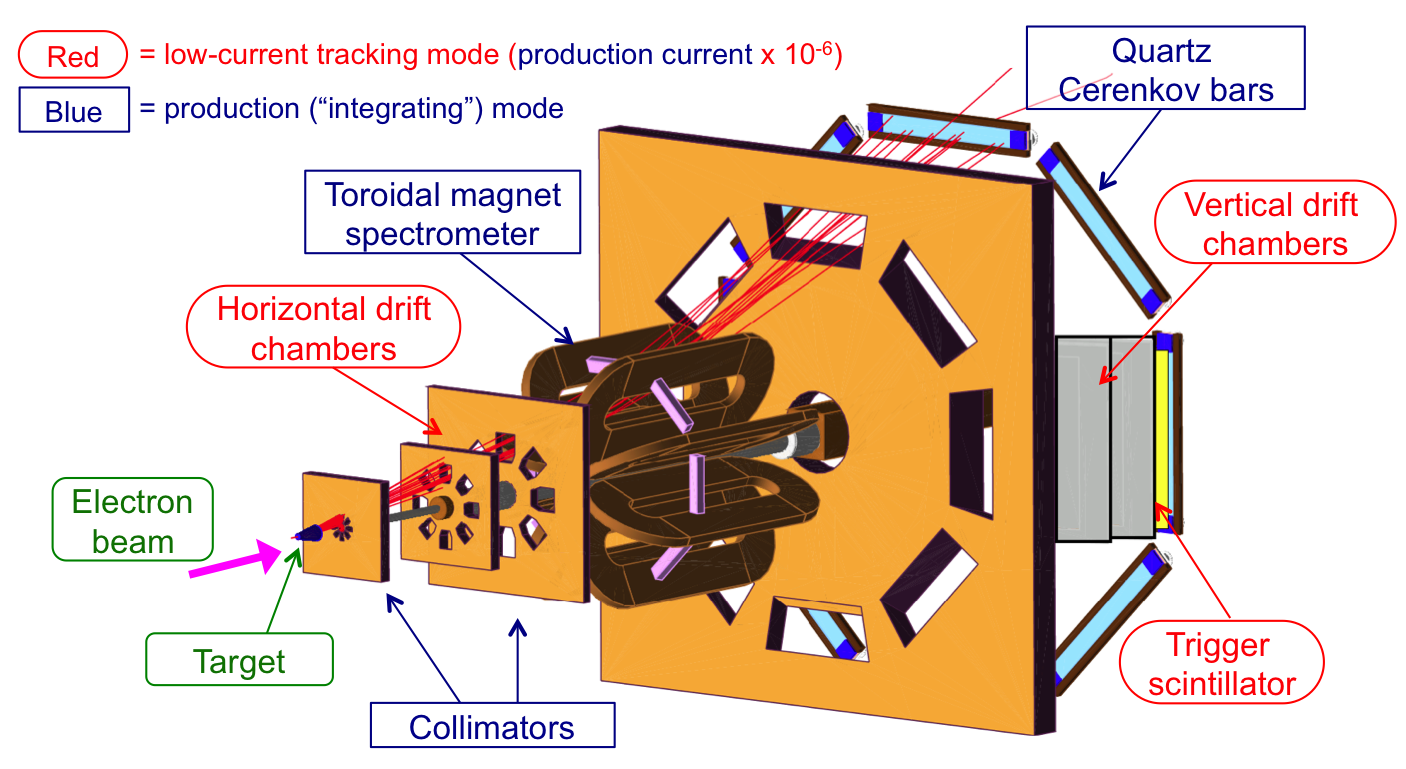
\includegraphics[width=9.0cm]{figures/qweak_schematics}
    \end{block}
    \end{column}
  \end{columns}

	\pause
Some text some text some text some text some text some text some text some text some text some text some text some text some text some text some text some text some text some text some text some text some text

\end{frame}



%%%%%%%%%%%%%%%%%%%%%%%%%%%%%%%%%%%%%%%%%%%%%%%%%%%%%%
%%%%%%%%%%%%%%%%%%%%%%%%%%%%%%%%%%%%%%%%%%%%%%%%%%%%%%

\section{\scshape Analysis}

%%%%%%%%%%%%%%%%%%%%%%%%%%%%%%%%%%%%%%%%%%%%%%%%%%%%%%
%%%%%%%%%%%%%%%%%%%%%%%%%%%%%%%%%%%%%%%%%%%%%%%%%%%%%%
\subsection{Transverse N-to-$\Delta$ Data Set}
\begin{frame}{Transverse N-to-$\Delta$ Data Set}

%\transblindshorizontal % Horizontal blinds pulled away
%\transblindsvertical % Vertical blinds pulled away
%\transboxin % Move to center from all sides
%\transboxout % Move to all sides from center
%\transdissolve % Slowly dissolve what was shown before
\transglitter % Glitter sweeps in specified direction
%\transslipverticalin % Sweeps two vertical lines in
%\transslipverticalout % Sweeps two vertical lines out
%\transhorizontalin % Sweeps two horizontal lines in
%\transhorizontalout % Sweeps two horizontal lines out
%\transwipe % Sweeps single line in specified direction
%\transduration{0.15} % Show slide specified number of seconds

%
%\begin{figure}[hp]
%	\begin{center}
%	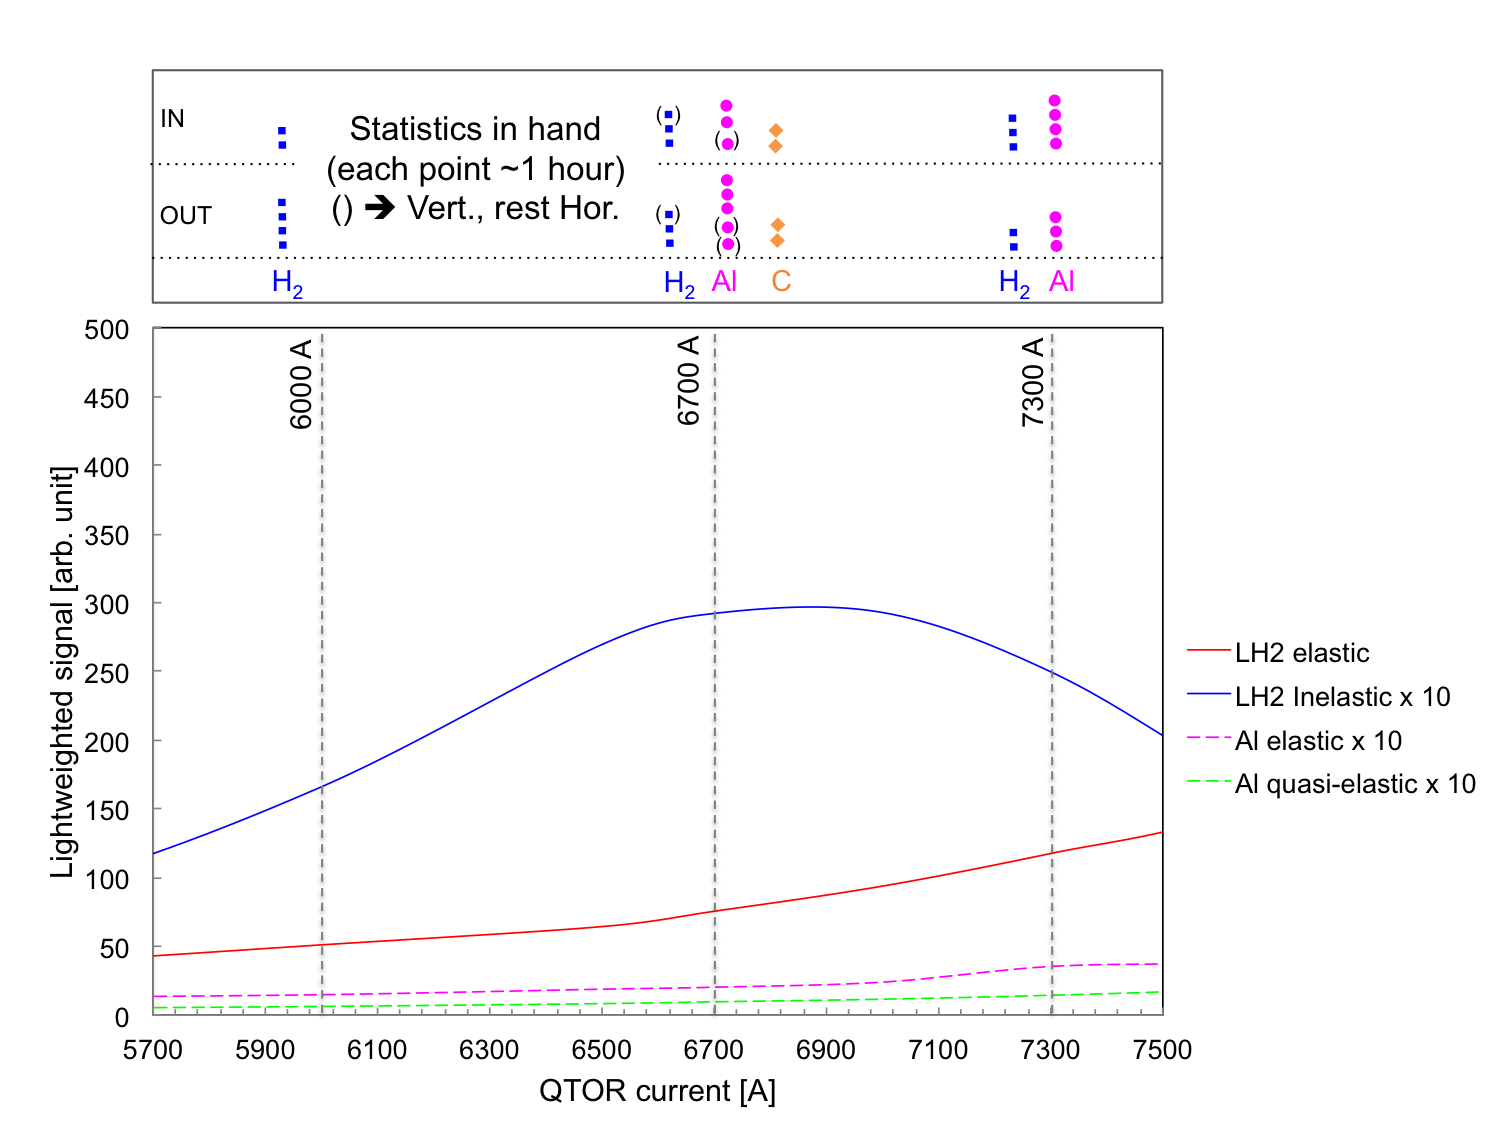
\includegraphics[width=9.0cm]{figures/transverseN2Delta}
%	\end{center}
%%	\caption[Schematic diagram of Jefferson Lab.]{Aerial view of Jefferson Lab (top left corner). Schematic diagram of Jefferson Lab. The elliptical region is the electron accelerator. Beam is accelerated by two linear accelerator namely North and South Linac. Three existing Halls A, B, C has been shown.}
%	\label{fig:jlab}
%\end{figure}

  \begin{columns}[T]
    \begin{column}{0.25\textwidth}
     \begin{block}{Your textblock}
	% Text here
	\pause
	Some text some text some text some text some text some text some text some text some text some text some.
    \end{block}
    \end{column}
    \begin{column}{0.8\textwidth}
    \begin{block}{}
	% Image included here
	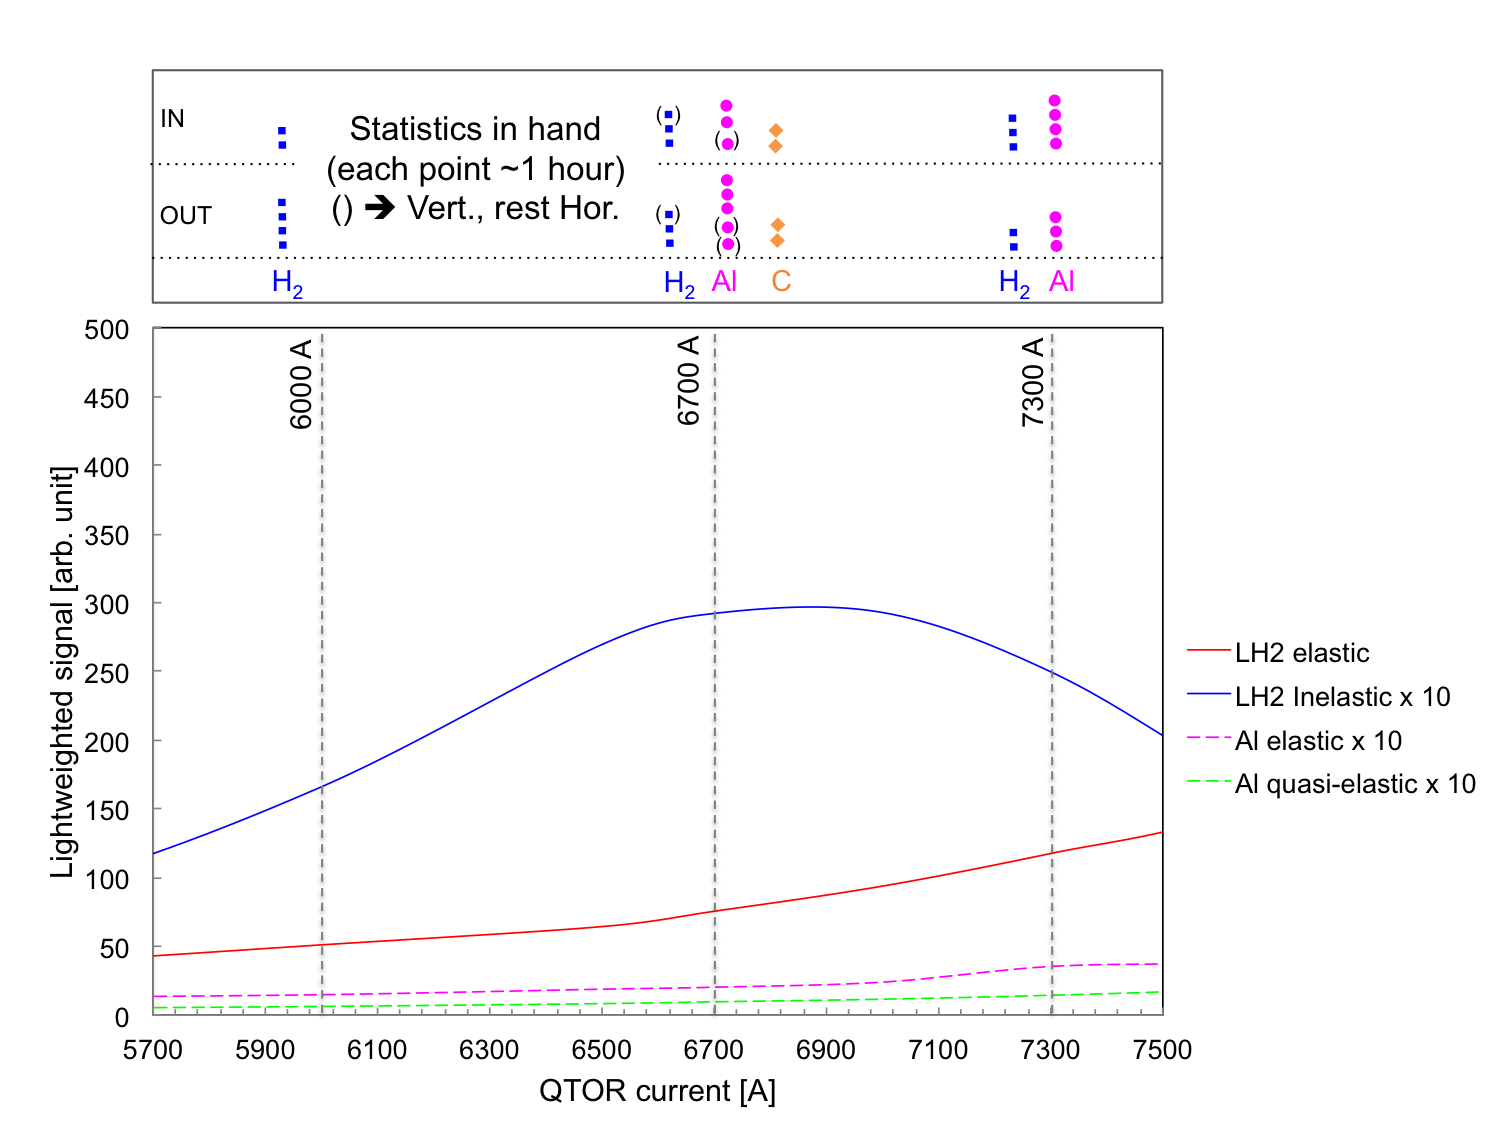
\includegraphics[width=9.0cm]{figures/transverseN2Delta}
    \end{block}
    \end{column}
  \end{columns}

	\pause
Some text some text some text some text some text some text some text some text some text some text some text some text some text some text some text some text some text some text some text some text some text

\end{frame}

%%%%%%%%%%%%%%%%%%%%%%%%%%%%%%%%%%%%%%%%%%%%%%%%%%%%%%
%%%%%%%%%%%%%%%%%%%%%%%%%%%%%%%%%%%%%%%%%%%%%%%%%%%%%%
\subsection{Transverse Asymmetries for N-to-$\Delta$ in Hydrogen}
\begin{frame}{Transverse Asymmetries for N-to-$\Delta$ in Hydrogen}

  \begin{columns}[T]
    \begin{column}{0.25\textwidth}
     \begin{block}{Your textblock}
	% Text here
	\pause
	Some text some text some text some text some text some text some text some text some text some text some.
    \end{block}
    \end{column}
    \begin{column}{0.8\textwidth}
    \begin{block}{}
	% Image included here
	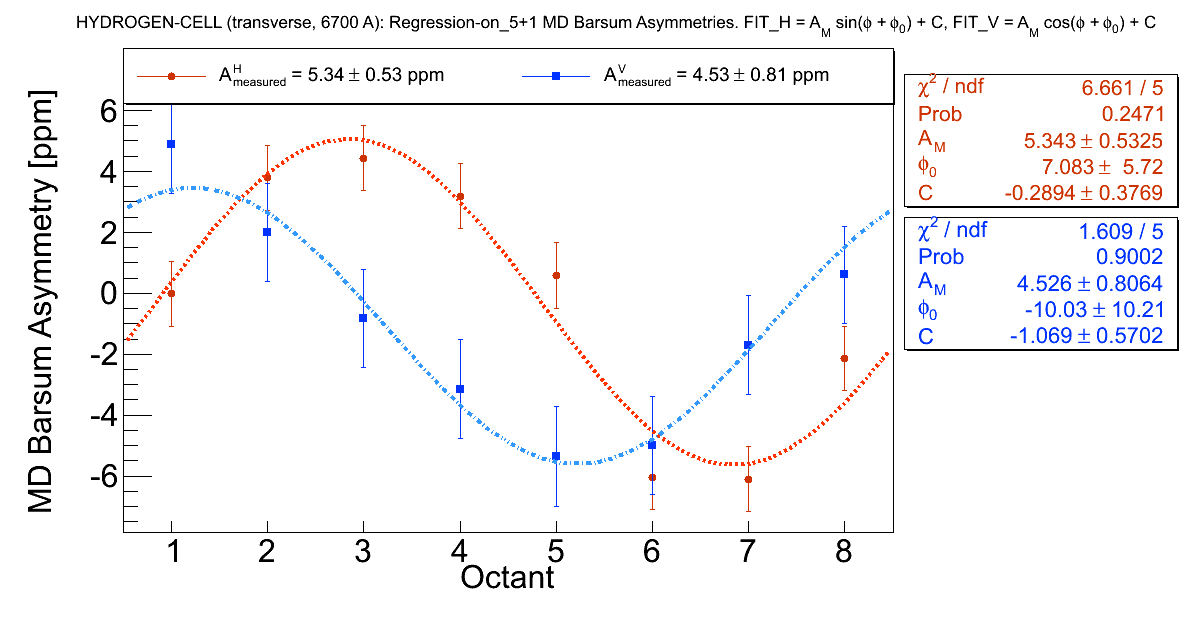
\includegraphics[width=9.0cm]{figures/n-to-delta_6700_combined_transverse_h_transverse_MD_HYDROGEN-CELL_regression_Barsum_off_slug_summary_plots_on_5+1}
    \end{block}
    \end{column}
  \end{columns}

	\pause
Some text some text some text some text some text some text some text some text some text some text some text some text some text some text some text some text some text some text some text some text some text

\end{frame}




%%%%%%%%%%%%%%%%%%%%%%%%%%%%%%%%%%%%%%%%%%%%%%%%%%%%%%
%%%%%%%%%%%%%%%%%%%%%%%%%%%%%%%%%%%%%%%%%%%%%%%%%%%%%%
\subsection{Summary of Uncertainties}


\begin{frame}{Summary of Uncertainties}


  \begin{columns}[T]
    \begin{column}{0.25\textwidth}
     \begin{block}{Your textblock}
	% Text here
	\pause
	Some text some text some text some text some text some text some text some text some text some text some.
    \end{block}
    \end{column}
    \begin{column}{0.8\textwidth}
    \begin{block}{}

%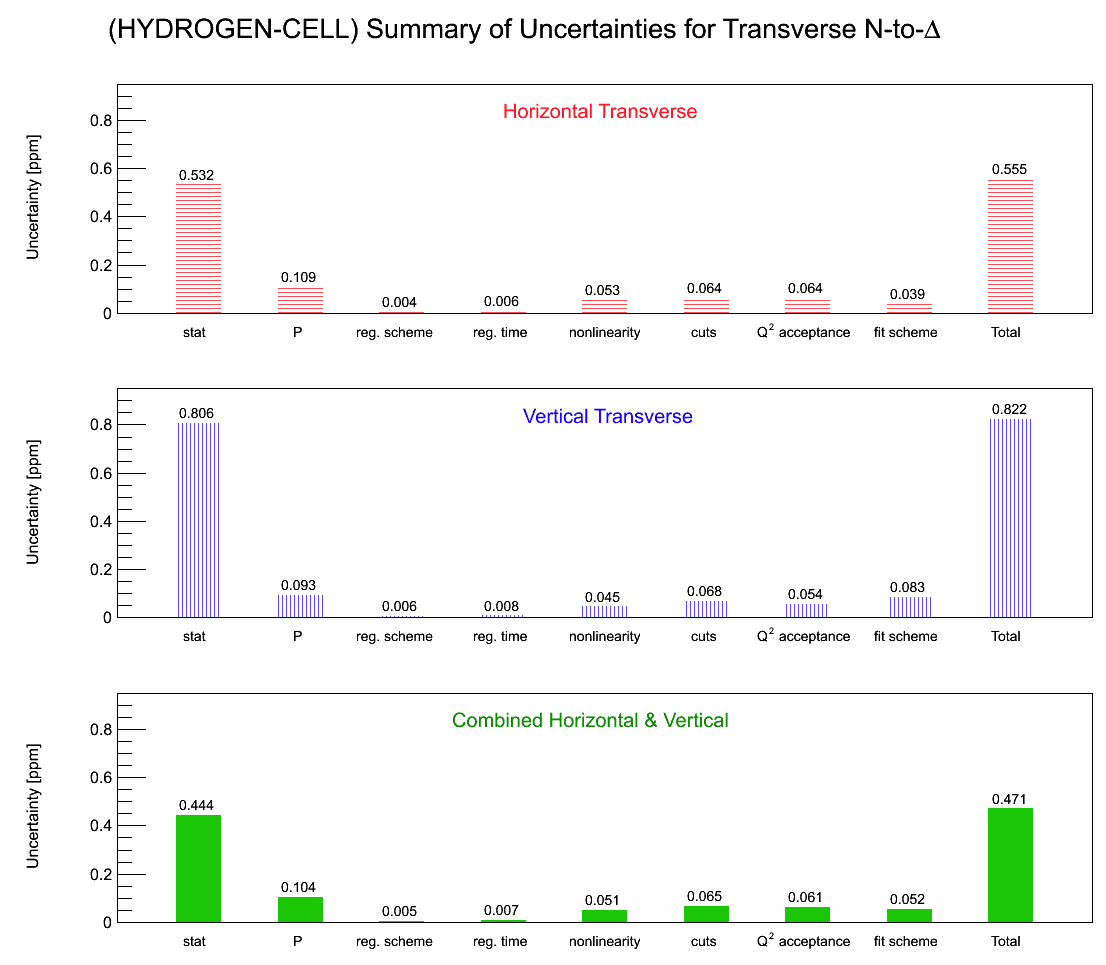
\includegraphics[width=8.0cm]{figures/n-to-delta_6700_HYDROGEN-CELL_MD_Error_Chart_run2_pass5}

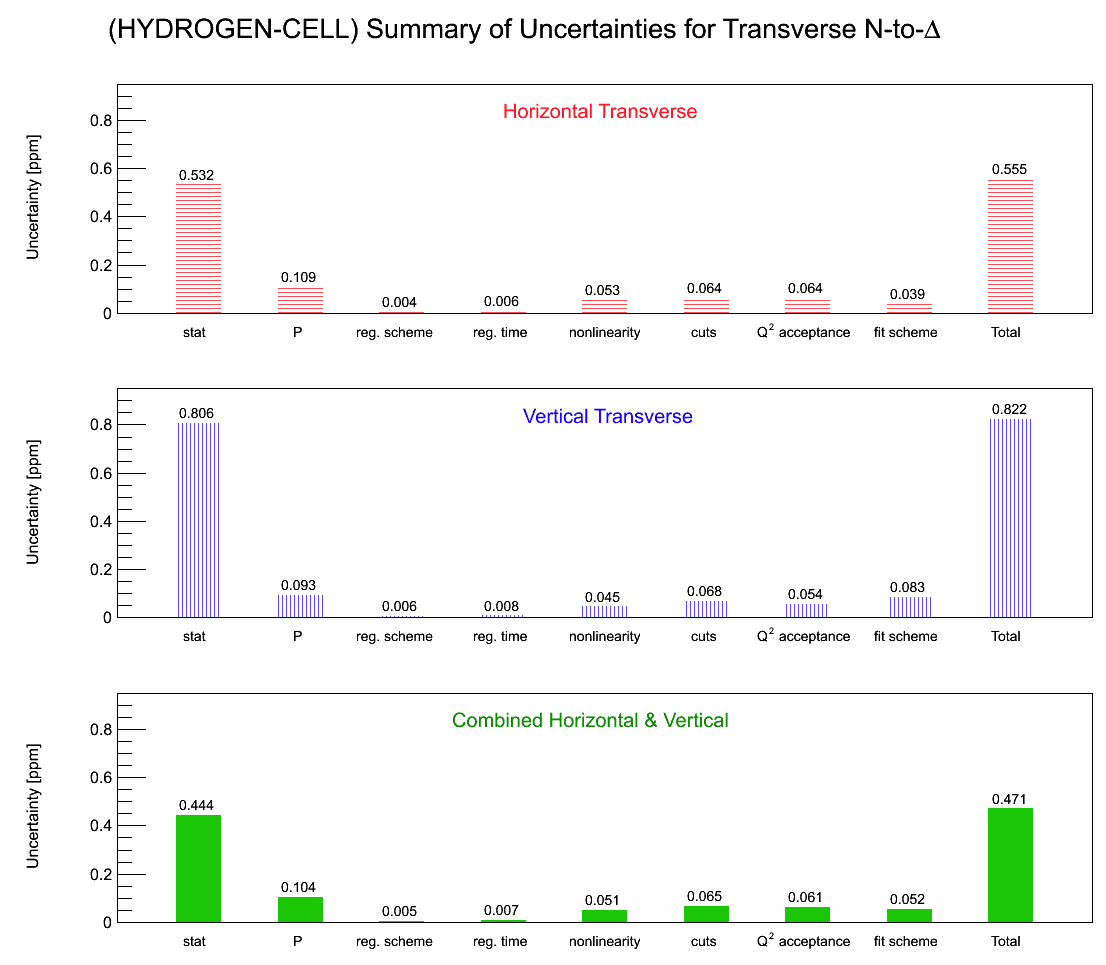
\includegraphics[width=9.0cm,trim=0cm 10cm 0cm 0cm, clip=true]{figures/n-to-delta_6700_HYDROGEN-CELL_MD_Error_Chart_run2_pass5}\\
%\pause
%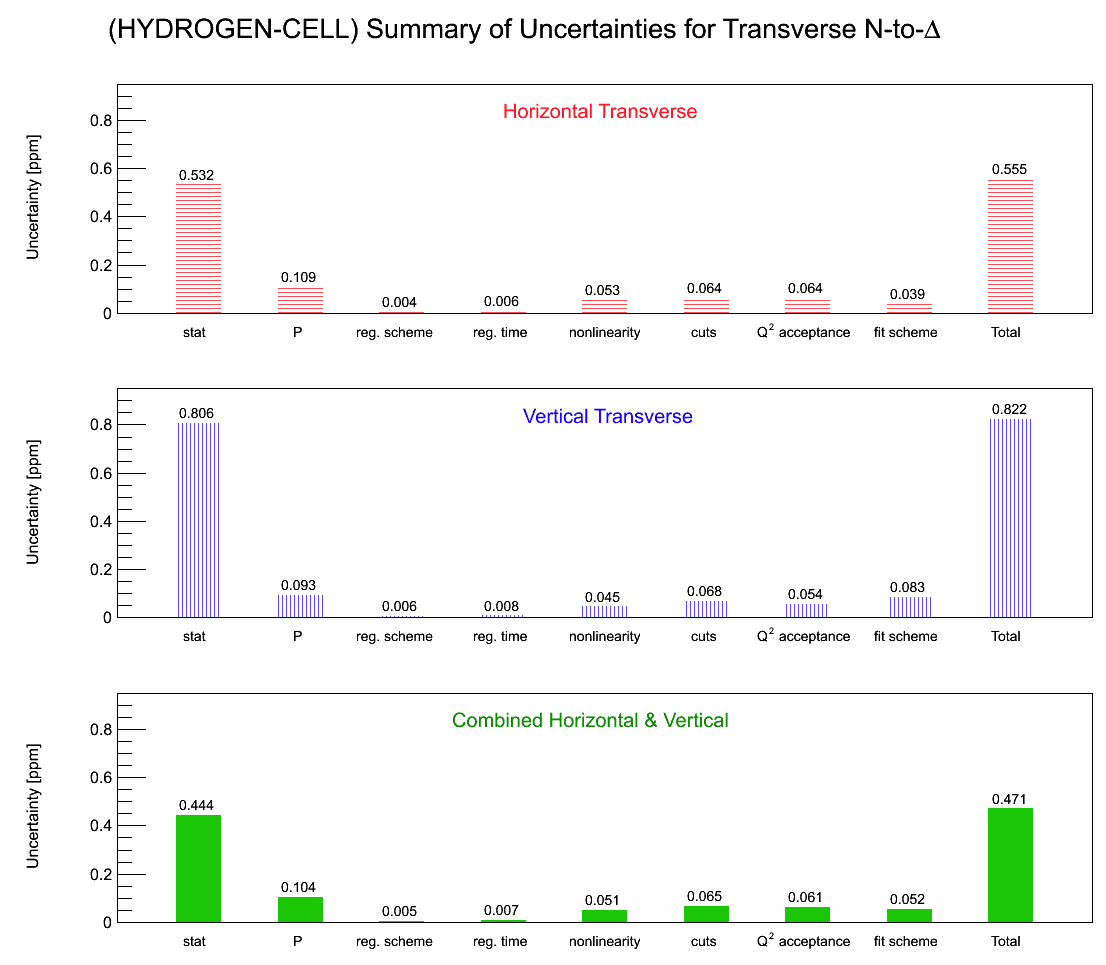
\includegraphics[width=8.5cm,trim=0cm 10cm 0cm 0cm, clip=true]{figures/n-to-delta_6700_HYDROGEN-CELL_MD_Error_Chart_run2_pass5}\\
%\pause
%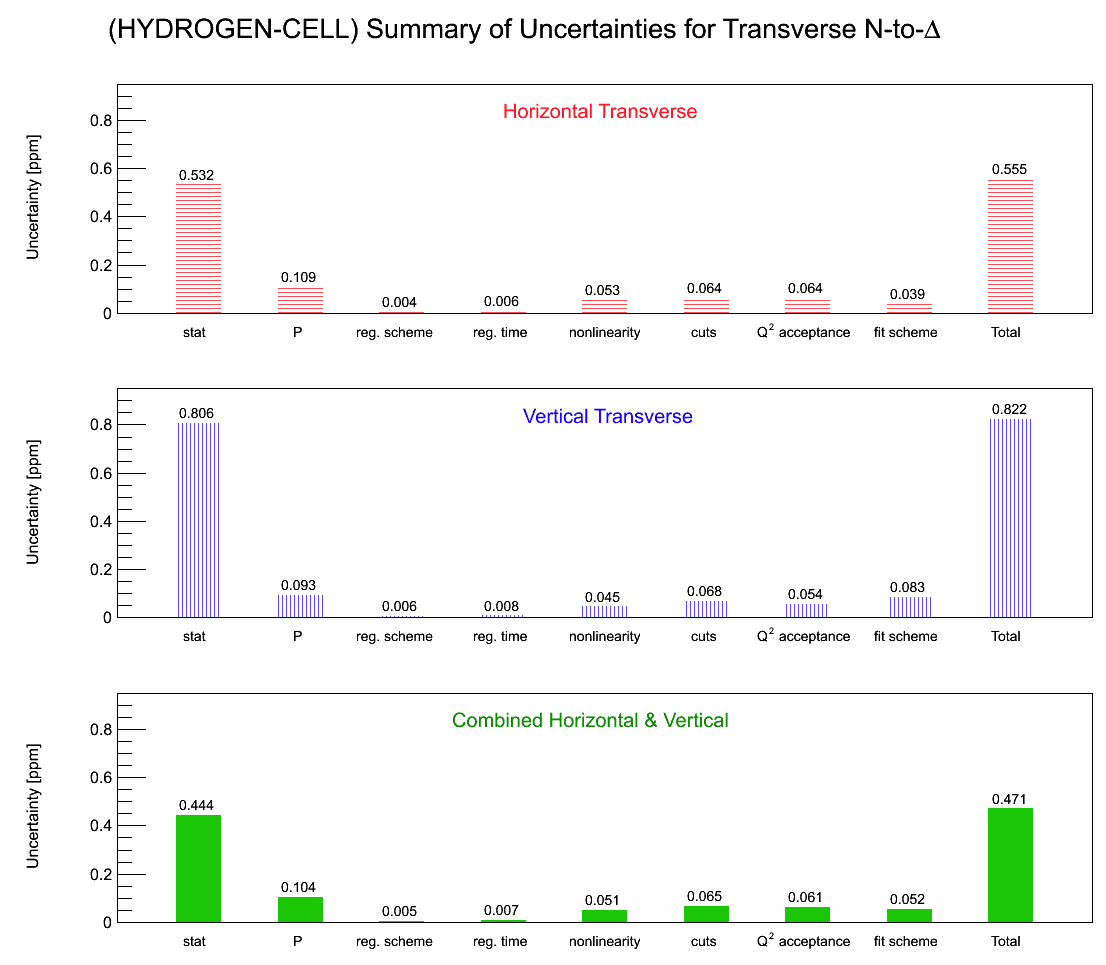
\includegraphics[width=8.5cm,trim=0cm 0cm 0cm 0cm, clip=true]{figures/n-to-delta_6700_HYDROGEN-CELL_MD_Error_Chart_run2_pass5}

%%\begin{tikzpicture}[every node/.style={fill,draw}]
%%%  \draw[line width=2mm,blue!50,line cap=round] (0,0) grid (3,2);
%%  \node[opacity=0.5] at (0.8,18.8) {Upper node};
%%  \node[draw opacity=0.8,fill opacity=0.2,text opacity=1]
%%    at (0.2,14.1) {Lower node};
%%\end{tikzpicture}

% \begin{tikzpicture}
%            \node[anchor=south west,inner sep=0] at (0,0) {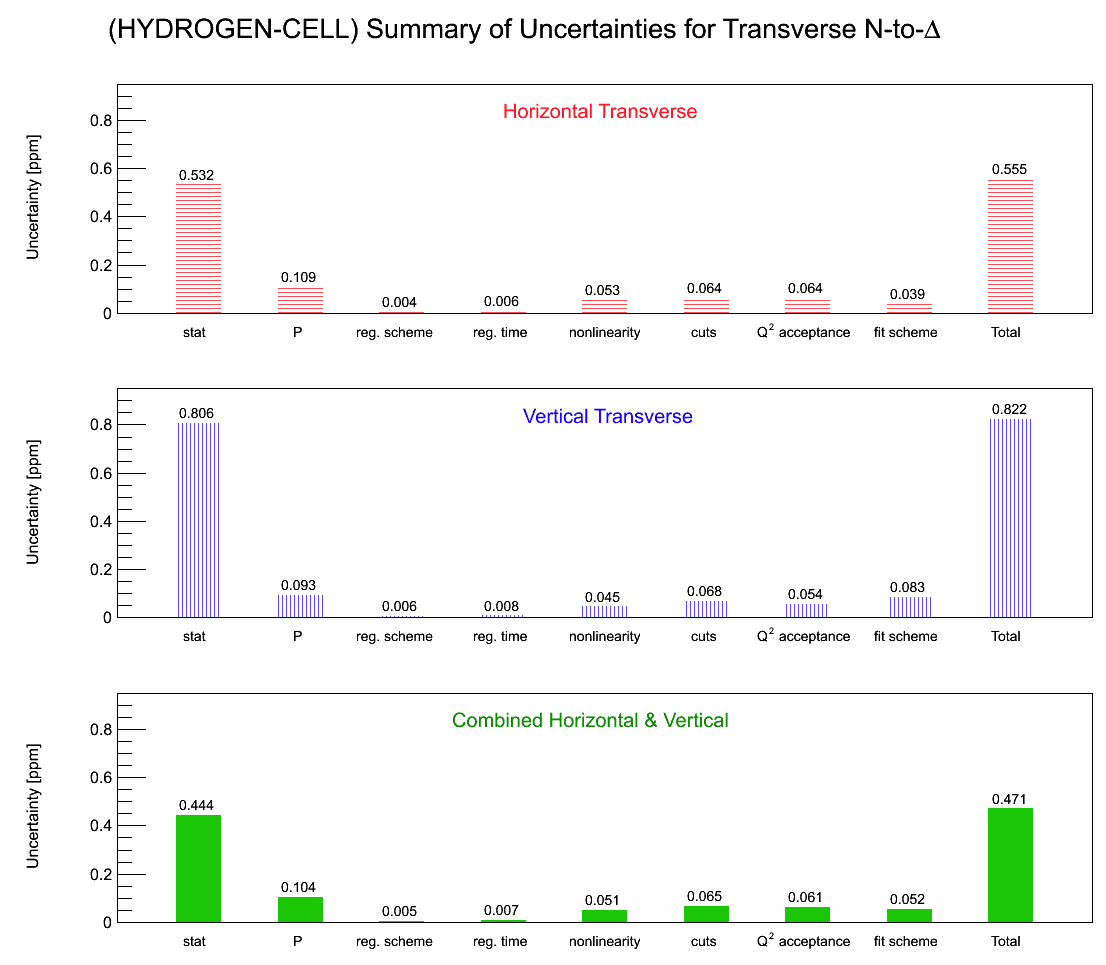
\includegraphics[width=8.5cm]{figures/n-to-delta_6700_HYDROGEN-CELL_MD_Error_Chart_run2_pass5}};
%            \draw<1>[red,ultra thick,rounded corners] (0.6,4) rectangle (\textheight-1cm,8.5);
%            \draw<2>[red,ultra thick,rounded corners] (2.7,14.1) rectangle (7.5,4.9);
%\end{tikzpicture}

%    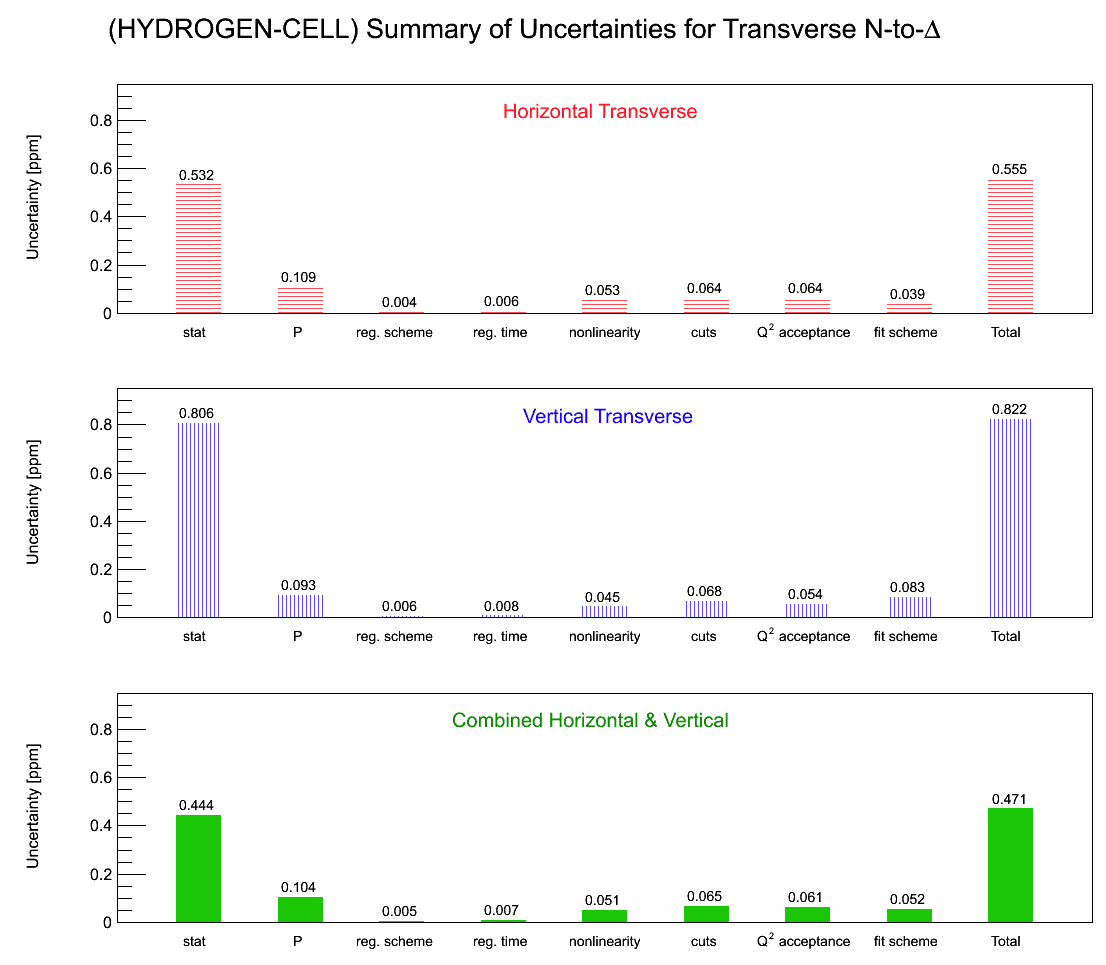
\includegraphics[clip,trim=0 90 120 0, width=8.5cm]{figures/n-to-delta_6700_HYDROGEN-CELL_MD_Error_Chart_run2_pass5}
%    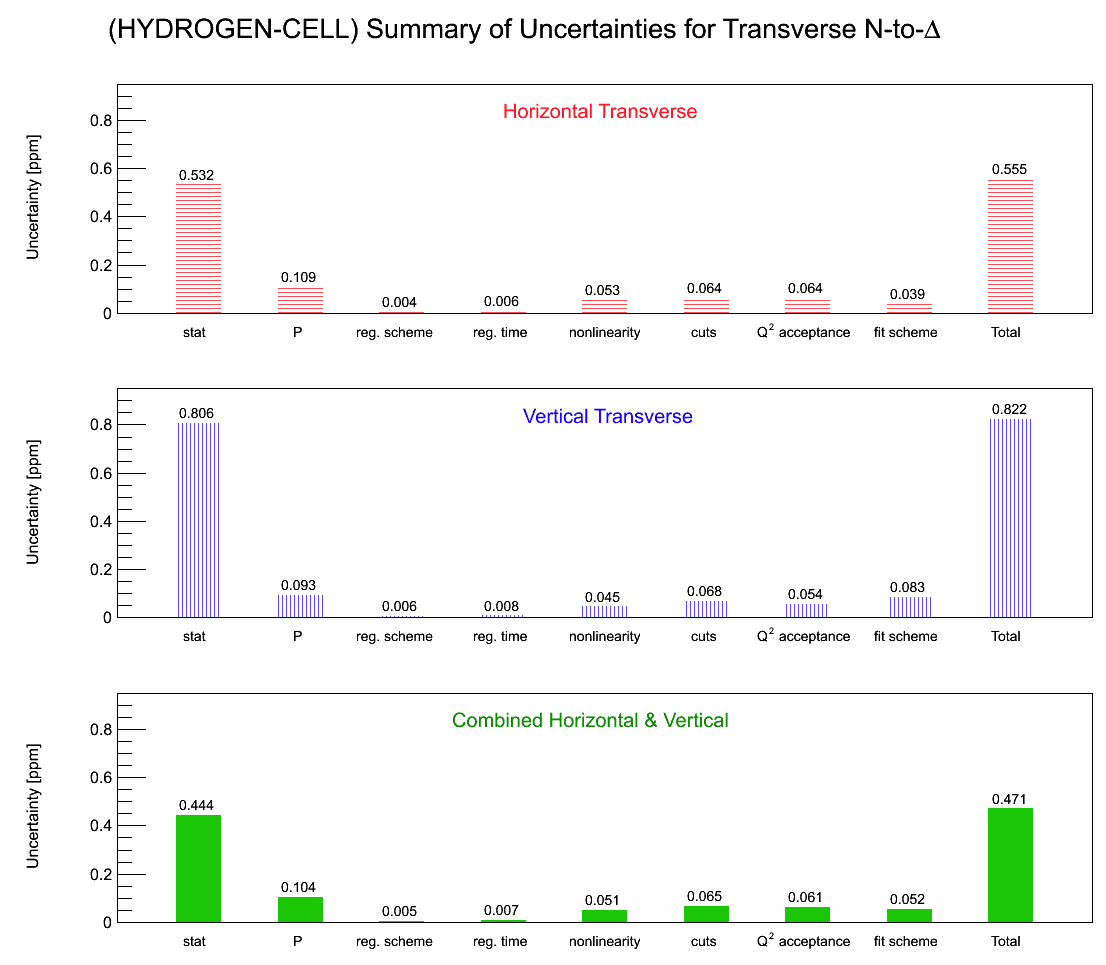
\includegraphics[width=8.5cm,clip,trim=0 0 325 20]{figures/n-to-delta_6700_HYDROGEN-CELL_MD_Error_Chart_run2_pass5}
%    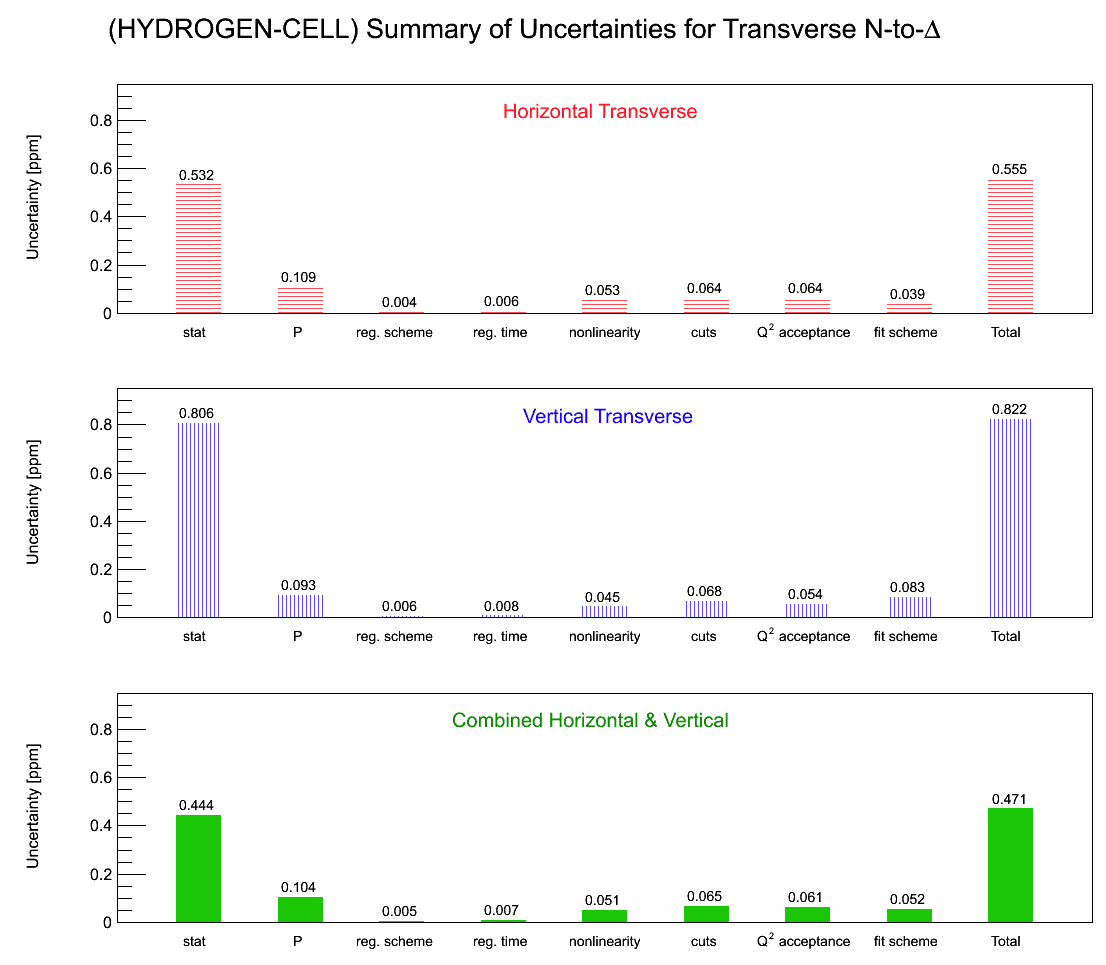
\includegraphics[clip,trim=125 90 0 0,width=8.5cm]{figures/n-to-delta_6700_HYDROGEN-CELL_MD_Error_Chart_run2_pass5}

    \end{block}
    \end{column}


  \end{columns}



	\pause
Some text some text some text some text some text some text some text some text some text some text some text some text some text some text some text some text some text some text some text some text some text

\end{frame}


%%%%%%%%%%%%%%%%%%%%%%%%%%%%%%%%%%%%%%%%%%%%%%%%%%%%%%
%%%%%%%%%%%%%%%%%%%%%%%%%%%%%%%%%%%%%%%%%%%%%%%%%%%%%%
\section{\scshape Results}
\subsection{Extraction of Physics Asymmetry}

\tikzstyle{every picture}+=[remember picture]
\everymath{\displaystyle}

\begin{frame}
\frametitle{Extracting Physics Asymmetry}

\tikzstyle{na} = [baseline=-.5ex]

\begin{equation*} \label{equ:eqAsym4}
        \tikz[baseline]{
            \node[anchor=base] (t1)
			{$A_{ep}$};\pause
			}
        \tikz[baseline]{
			\node[anchor=base] (t2)
			{$ = R_{total}$};  \pause
        		}
        \tikz[baseline]{
			\node[anchor=base] (t3)
			{$\left[  \frac{A_{M}/P \pause - \displaystyle\sum_{i=1}^{4} f_{i}A_{i} }{1- \displaystyle\sum_{i=1}^{4} f_{i} } \right]$};  %\pause
        } 
\end{equation*}


\begin{itemize}[<+-| alert@+>]
    \item Polarization
        \tikz[na] \node[coordinate] (n1) {};
            \item Multiplicative corrections $R_{total}$ = $R_{RC}R_{Det}R_{Bin}R_{Q^{2}}$\\
            Radiative correction $R_{RC}$\\
            Detector bias correction $R_{Det}$\\
            Bis centering correction $R_{Bin}$\\
            $Q^{2}$ correction $R_{Q^{2}}$\\
        \tikz[na]\node [coordinate] (n2) {};
    \item Background corrections \\
    			Al. window correction $A_{b1}$ = ppm, $f_{b1}$ = , $c_{b1}$ = ppm\\
    			Beamline background $A_{b2}$ = ppm, $f_{b2}$ = , $c_{b2}$ = ppm\\
    			Other neutral $A_{b3}$ = ppm, $f_{b3}$ = , $c_{b3}$ = ppm\\
    			Inelastic correction $A_{b4}$ = ppm, $f_{b4}$ = , $c_{b4}$ = ppm\\
        \tikz[na]\node [coordinate] (n3) {};

\end{itemize}

\begin{tikzpicture}[overlay]
        \path[->]<1-> (n1) edge [bend left] (t1);
        \path[->]<2-> (n2) edge [bend right] (t2);
        \path[->]<3-> (n3) edge [out=0, in=-90] (t3);
\end{tikzpicture}


\end{frame}


%%%%%%%%%%%%%%%%%%%%%%%%%%%%%%%%%%%%%%%%%%%%%%%%%%%%%%
%%%%%%%%%%%%%%%%%%%%%%%%%%%%%%%%%%%%%%%%%%%%%%%%%%%%%%
\subsection{\scshape Results}

%\begin{landscape}
\fontsize{6pt}{7.2}\selectfont

\begin{center}

%\begin{flushleft}
\begin{table}[h]
\begin{center}
  \begin{tabular}{@{} c @{}| @{} c  @{} c @{}|@{} c @{} c @{} |@{} c @{} c @{}| @{} c @{}}
    \hline
    Quantity	&	&	Asymmetry [ppm]	& 	& Dilution & Cor. & $c_{i}=A_{bi}f_{bi}$ & Ref.		\\
	\hline
	Aluminum window & $A_{b1}$ & 8.431 $\pm$ 0.985 & $f_{b1}$ & 0.033 $\pm$ 0.002 & $c_{b1}$ & 0.033 $\pm$ 0.002 &	\href{https://qweak.jlab.org/elog/Analysis+&+Simulation/451}{ELOG 451 (Analysis)}\cite{website:elog_adesh} 
	\\
	Beamline scattering & $A_{b2}$ & 0.000 $\pm$ 0.000 & $f_{b2}$ & 0.033 $\pm$ 0.002 & $c_{b1}$ & 0.033 $\pm$ 0.002 & \href{https://qweak.jlab.org/doc-private/ShowDocument?docid=1655}{DocDB 1655} \cite{buddhini_transverse_technote}	
	\\
	Other neutrals & $A_{b3}$ & 0.000 $\pm$ 0.000 	& $f_{b3}$ & 0.033 $\pm$ 0.002 & $c_{b1}$ & 0.033 $\pm$ 0.002 & 	\href{https://qweak.jlab.org/doc-private/ShowDocument?docid=1655}{DocDB 1655} \cite{buddhini_transverse_technote}	
	\\	
	Inelastics & $A_{b4}$ & -5.305 $\pm$ 0.166 & $f_{b4}$ & 0.033 $\pm$ 0.002 & $c_{b1}$ & 0.033 $\pm$ 0.002 &	\href{https://qweak.jlab.org/doc-private/ShowDocument?docid=1655}{DocDB 1655} \cite{buddhini_transverse_technote}	
	\\
    \hline
  	\end{tabular}
  	\caption[Background correction table.]{Background correction table.}
  \label{tabPhysicsAsymInput}
\end{center}
\end{table}
%\end{flushleft}

\end{center}

%\end{frame}
%
%
%\begin{frame}{Frame 1}
%

\begin{table}[h]
\begin{center}
  \begin{tabular}{ c  c  c  c  c  c  c }
    \hline
    Quantity 		&	&	Value	&	&	& &  Reference		\\
	\hline
	Inelastic measured asymmetry & $A^{in}_{M}$ &	4.789 $\pm$ 0.844 & ppm & & & This analysis\\

	Polarization & P & 	0.879 $\pm$ 0.018 & &	& & \href{https://qweak.jlab.org/doc-private/ShowDocument?docid=1655}{DocDB 1655} \cite{buddhini_transverse_technote}	\\

	Aluminum asymmetry & $A_{b1}$ & 8.431 $\pm$ 0.985 & ppm & $f_{b1}$ & 0.033 $\pm$ 0.002 &	This analysis\\
	
%	Aluminum dilution factor & $f_{b1}$ & 0.033 $\pm$ 0.002 & &	\href{https://qweak.jlab.org/elog/Analysis+&+Simulation/451}{ELOG 451 (Analysis)}\cite{website:elog_adesh}	\\

%	Aluminum asymmetry radiative correction & $R^{A}_{b1}$ & 1.000 $\pm$ 0.000 &		&	Place holder	\\

	QTOR transport channel & $A_{b2}$ & 0.000 $\pm$ 0.000 & ppm	& $f_{b1}$ & 0.033 $\pm$ 0.002 & \href{https://qweak.jlab.org/doc-private/ShowDocument?docid=1655}{DocDB 1655} \cite{buddhini_transverse_technote}	\\
	
%	QTOR transport channel neutral dilution & $f_{b2}$ & 0.724 $\pm$ 0.004 & &	\href{https://qweak.jlab.org/elog/Analysis+&+Simulation/451}{ELOG 451 (Analysis)}\cite{website:elog_adesh}	\\

	Beamline background & $A_{b3}$ & 0.000 $\pm$ 0.000 & ppm	& $f_{b1}$ & 0.033 $\pm$ 0.002 & 	\href{https://qweak.jlab.org/doc-private/ShowDocument?docid=1655}{DocDB 1655} \cite{buddhini_transverse_technote}	\\
	
%	Beamline background dilution & $f_{b3}$ & 0.724 $\pm$ 0.004 & &	\href{https://qweak.jlab.org/elog/Analysis+&+Simulation/451}{ELOG 451 (Analysis)}\cite{website:elog_adesh}	\\
	
	Elastic asymmetry & $A_{b4}$ & -5.305 $\pm$ 0.166 & ppm	& $f_{b1}$ & 0.033 $\pm$ 0.002 &	\href{https://qweak.jlab.org/doc-private/ShowDocument?docid=1655}{DocDB 1655} \cite{buddhini_transverse_technote}	\\
	
%	Elastic dilution factor & $f_{b4}$ & 0.724 $\pm$ 0.004 & &	\href{https://qweak.jlab.org/elog/Analysis+&+Simulation/451}{ELOG 451 (Analysis)}\cite{website:elog_adesh}	\\

%	Elastic asymmetry radiative correction & $R^{A}_{b4}$ & 1.000 $\pm$ 0.000 &		&	Place holder	\\
%
%	EM radiative correction & $R_{RC}$ & 1.000 $\pm$ 0.000 &		&	Place holder	\\
%
%	Detector bias correction & $R_{Det}$ & 1.000 $\pm$ 0.000 &		&	Place holder	\\

    \hline
  	\end{tabular}
  	\caption[Input table.]{Input table.}
  \label{tabPhysicsAsymInput}
\end{center}
\end{table}


%\end{landscape}

%\end{frame}


%%%%%%%%%%%%%%%%%%%%%%%%%%%%%%%%%%%%%%%%%%%%%%%%%%%%%%
%%%%%%%%%%%%%%%%%%%%%%%%%%%%%%%%%%%%%%%%%%%%%%%%%%%%%%
\section{\scshape Summary}
\subsection{Summary}
\begin{frame}{Summary}


%\fontsize{10pt}{7.2}\selectfont
%Summary

\begin{block}{Summary}

\fontsize{8pt}{7.2}\selectfont
\begin{itemize}
\item The uncertainty in measured N-to-$\Delta$ transverse asymmetry is dominated by statistics for in hydrogen. Next largest contribution comes from polarization. Most other systematic uncertainties are under control. 
\item A conservative estimate of extracted physics asymmetry using preliminary background asymmetries and dilutions is A$_{PHYS}^{in}$ = 41.05 $\pm$ 7.90 ppm. Largest contribution in the uncertainties is from elastic dilution.
\end{itemize}

\end{block}

\pause

\hfill
%\fontsize{10pt}{7.2}\selectfont
%To Do

\begin{block}{To Do}

\fontsize{8pt}{7.2}\selectfont
\begin{itemize}
\item Beamline background, detector bias correction, radiative correction etc.
\item Update dilution factors.
\item Quantify impact of these results on the PV N-to-$\Delta$ measurement and talk to theoretician for model calculation.
\end{itemize}

\end{block}

\end{frame}

%%%%%%%%%%%%%%%%%%%%%%%%%%%%%%%%%%%%%%%%%%%%%%%%%%%%%%
\appendix
%\newcounter{finalframe}
%\setcounter{finalframe}{\value{framenumber}}
%% Backup frames
%\setcounter{framenumber}{\value{finalframe}}














%%%%%%%%%%%%%%%%%%%%%%%%%%%%%%%%%%%%%%%%%%%%%%%%%%%%%%
%%%%%%%%%%%%%%%%%%%%%%%%%%%%%%%%%%%%%%%%%%%%%%%%%%%%%%
%%%%%%%%%%%%%%%%%%%%%%%%%%%%%%%%%%%%%%%%%%%%%%%%%%%%%%
%%%%%%%%%%%%%%%%%%%%%%%%%%%%%%%%%%%%%%%%%%%%%%%%%%%%%%

\section{\scshape Backup Slides}
\begin{frame}[noframenumbering]{frame 1}

\end{frame}
%%%%%%%%%%%%%%%%%%%%%%%%%%%%%%%%%%%%%%%%%%%%%%%%%%%%%%

\section{\scshape Backup}
\subsection{frame 12}
\begin{frame}[noframenumbering]{frame 1}
\begin{itemize}
\item Item A
\item Item B
\begin{itemize}
\item Subitem 1
\item Subtem 2
\end{itemize}
\item Item C
\end{itemize}
\end{frame}

\begin{frame}[noframenumbering]{frame 2}
\begin{itemize}
\item Item A
\item Item B
\begin{itemize}
\item Subitem 1
\item Subtem 2
\end{itemize}
\item Item C
\end{itemize}

\frame{
\hyperlink{equ:qweak6}{\beamergotobutton{Jump to Theorem ~\ref{equ:qweak6} }}
\hypertarget{equ:qweak6}{}
}

\end{frame}

%%%%%%%%%%%%%%%%%%%%%%%%%%%%%%%%%%%%%%%%%%%%%%%%%%%%%%
%%%%%%%%%%%%%%%%%%%%%%%%%%%%%%%%%%%%%%%%%%%%%%%%%%%%%%
\subsection{frame 3}
\begin{frame}{frame 3}

\begin{table}
\caption{Table}
\begin{tabular}{l c c c c c c}
\hline \hline
No.  & {Ordinary} & {Blue} & {Pink} & {Yellow} & {Green} & {RCM}\\
\hline
\only<1,3>{
&\multicolumn{6}{c}{$\alpha$=0.05}\\
H=2     &     95.0 &    75.3    &   75.7    &   79.5    &   72.0    &\\
H=3 & 95.6 &    87.0    &   87.3    &   87.6    &   85.2    & \\
H=4 & 95.0 &    91.6    &   91.9    &   90.3    &   90.2    & 93.3\\
H=5 & 95.2 &    93.5    &   93.7    &   91.3    &   91.8    & 94.3\\
H=6 & 94.9 &    93.8    &   94.1    &   92.6    &   92.8    & 94.7 \\[-\normalbaselineskip]
}\only<3>{\\}
\only<2,3>{
&\multicolumn{6}{c}{$\alpha$=0.5}\\
H=2 & 95.0  &   91.4    &   91.2    &   79.5    &   99.9    &   \\
H=3 & 95.6  &   95.1    &   95.1    &   87.6    &   95.1    &   \\
H=4 & 95.0  &   94.8    &   94.8    &   90.3    &   93.5    & 95.5  \\
H=5 & 95.2  &   95.1    &   95.2    &   91.3    &   93.1    & 95.9  \\
H=6 & 94.9  &   94.8    &   94.8    &   92.6    &   93.4    & 95.5 \\[-\normalbaselineskip]
}
\\\hline
\end{tabular}
\end{table}

%\animategraphics[controls]{1}{image}{1}{2}

\end{frame}

%%%%%%%%%%%%%%%%%%%%%%%%%%%%%%%%%%%%%%%%%%%%%%%%%%%%%%
%%%%%%%%%%%%%%%%%%%%%%%%%%%%%%%%%%%%%%%%%%%%%%%%%%%%%%
\section{\scshape Methodology}
\subsection{frame 4}
\begin{frame}{frame 4}

\only<2>{
	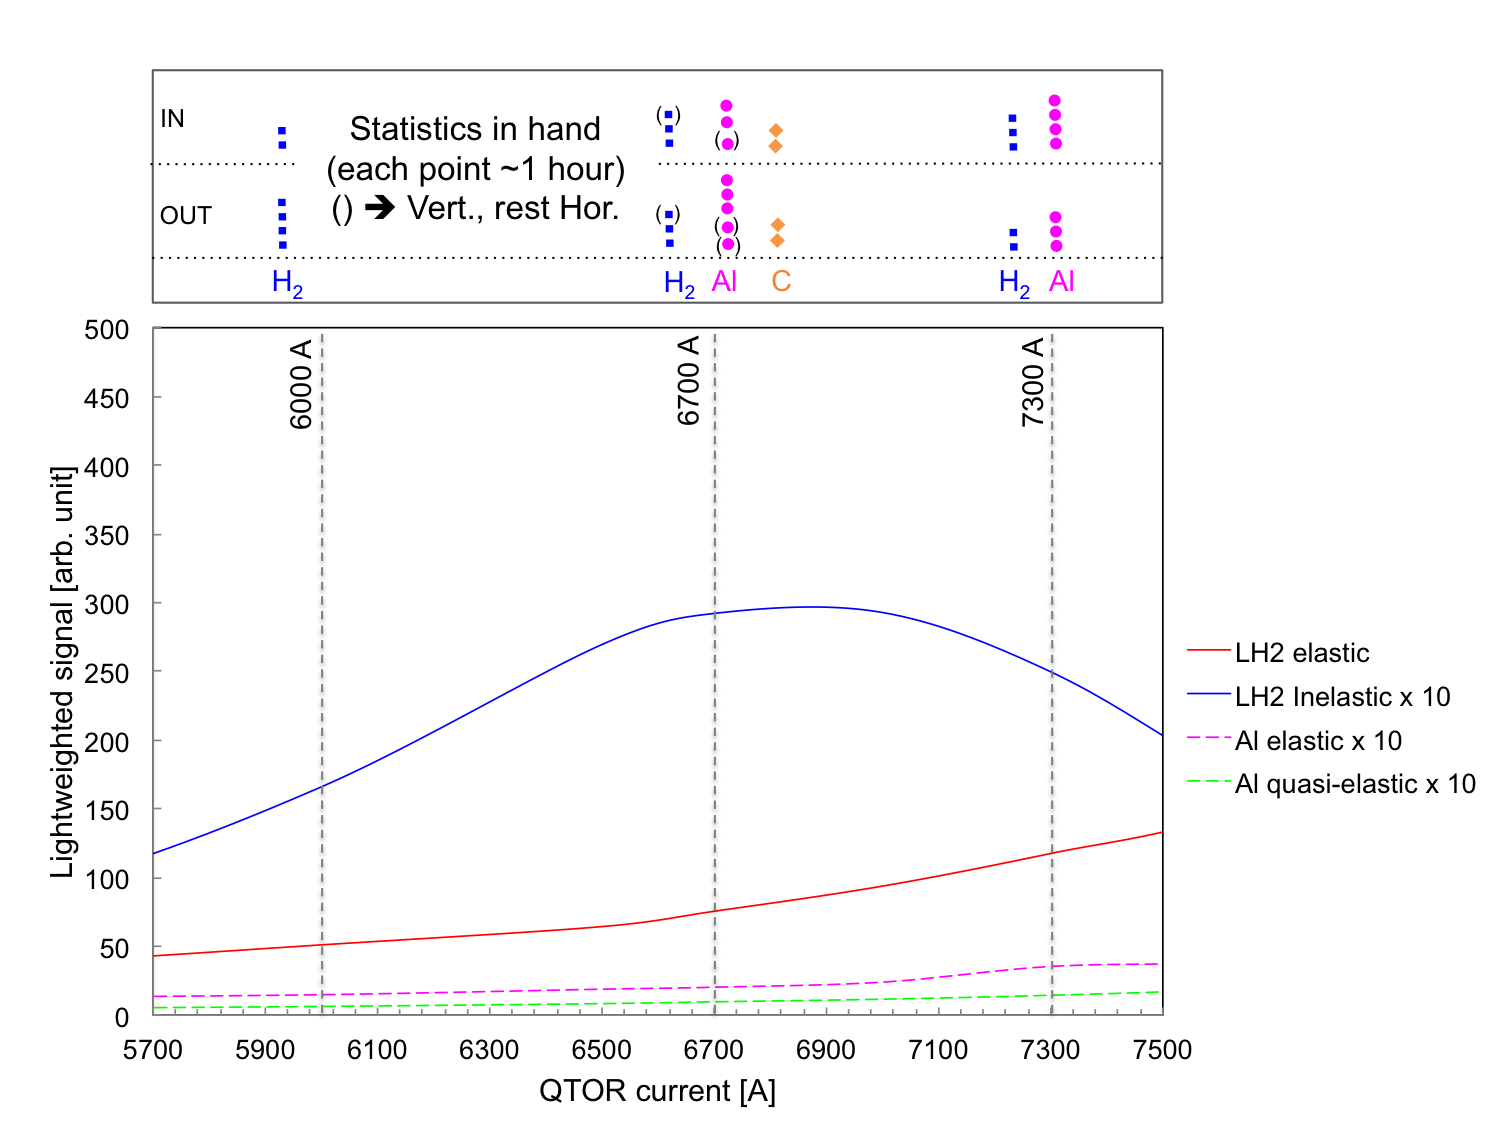
\includegraphics[width=5.0cm]{figures/transverseN2Delta}
	}
\hspace{-0.17em}\only<3>{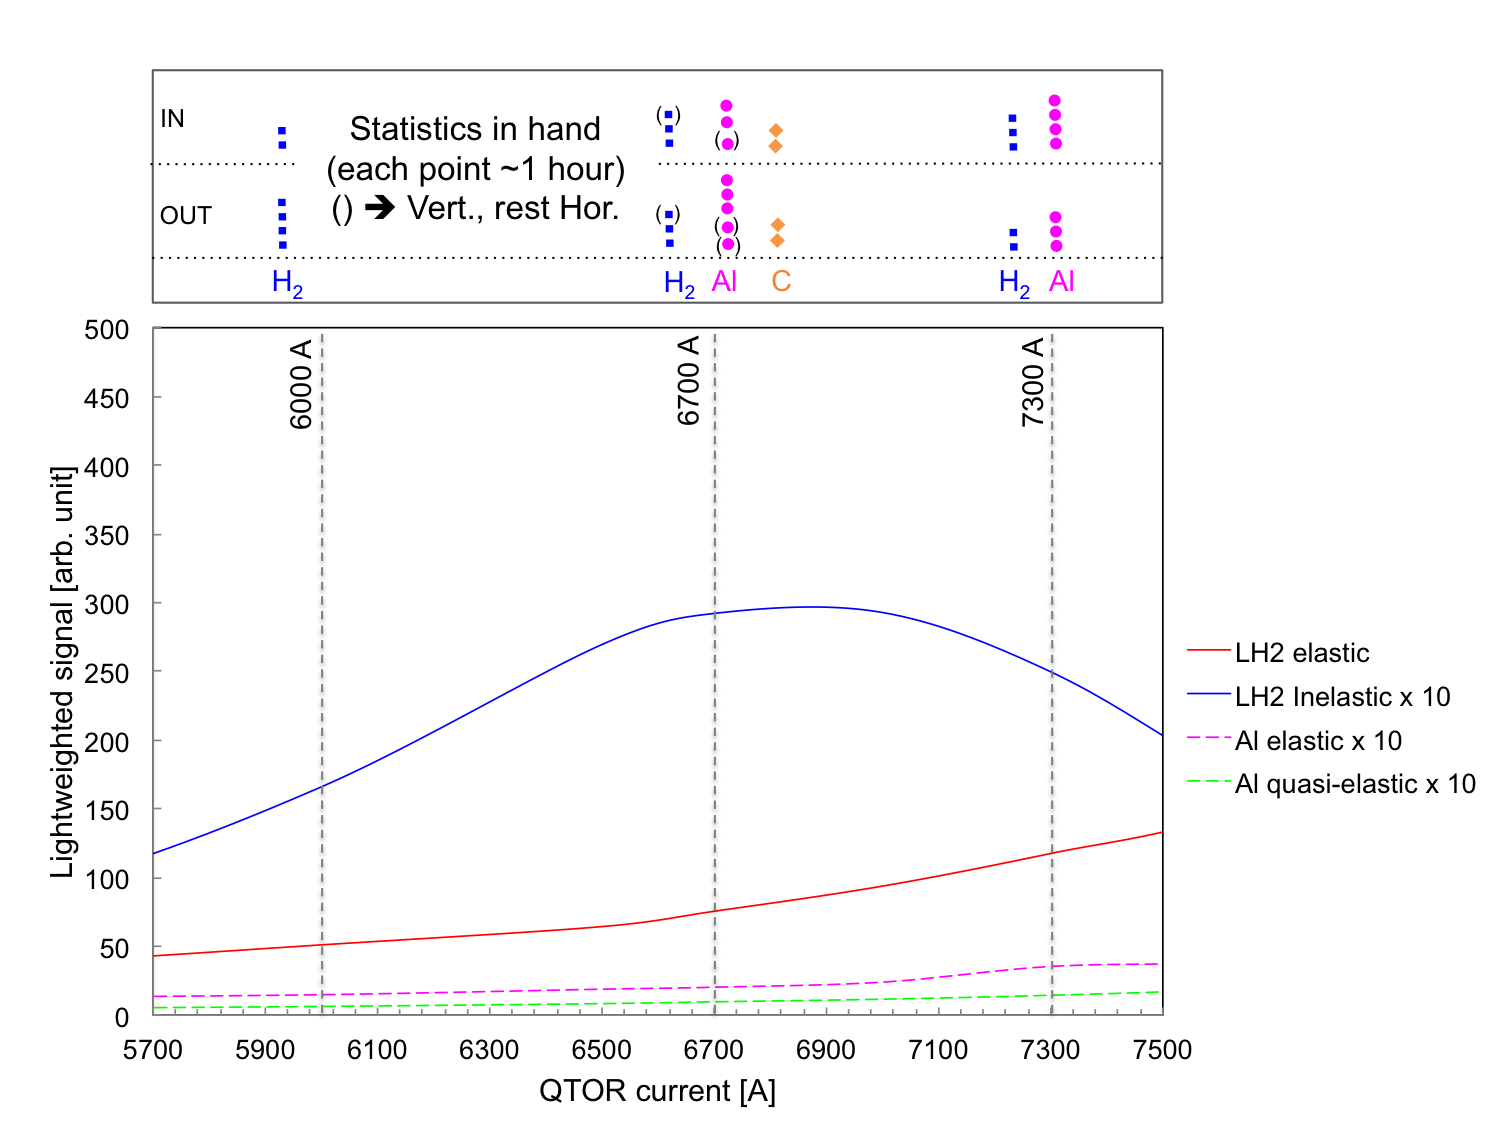
\includegraphics[width=5.0cm]{figures/transverseN2Delta}}
\hspace{-0.34em}\only<4>{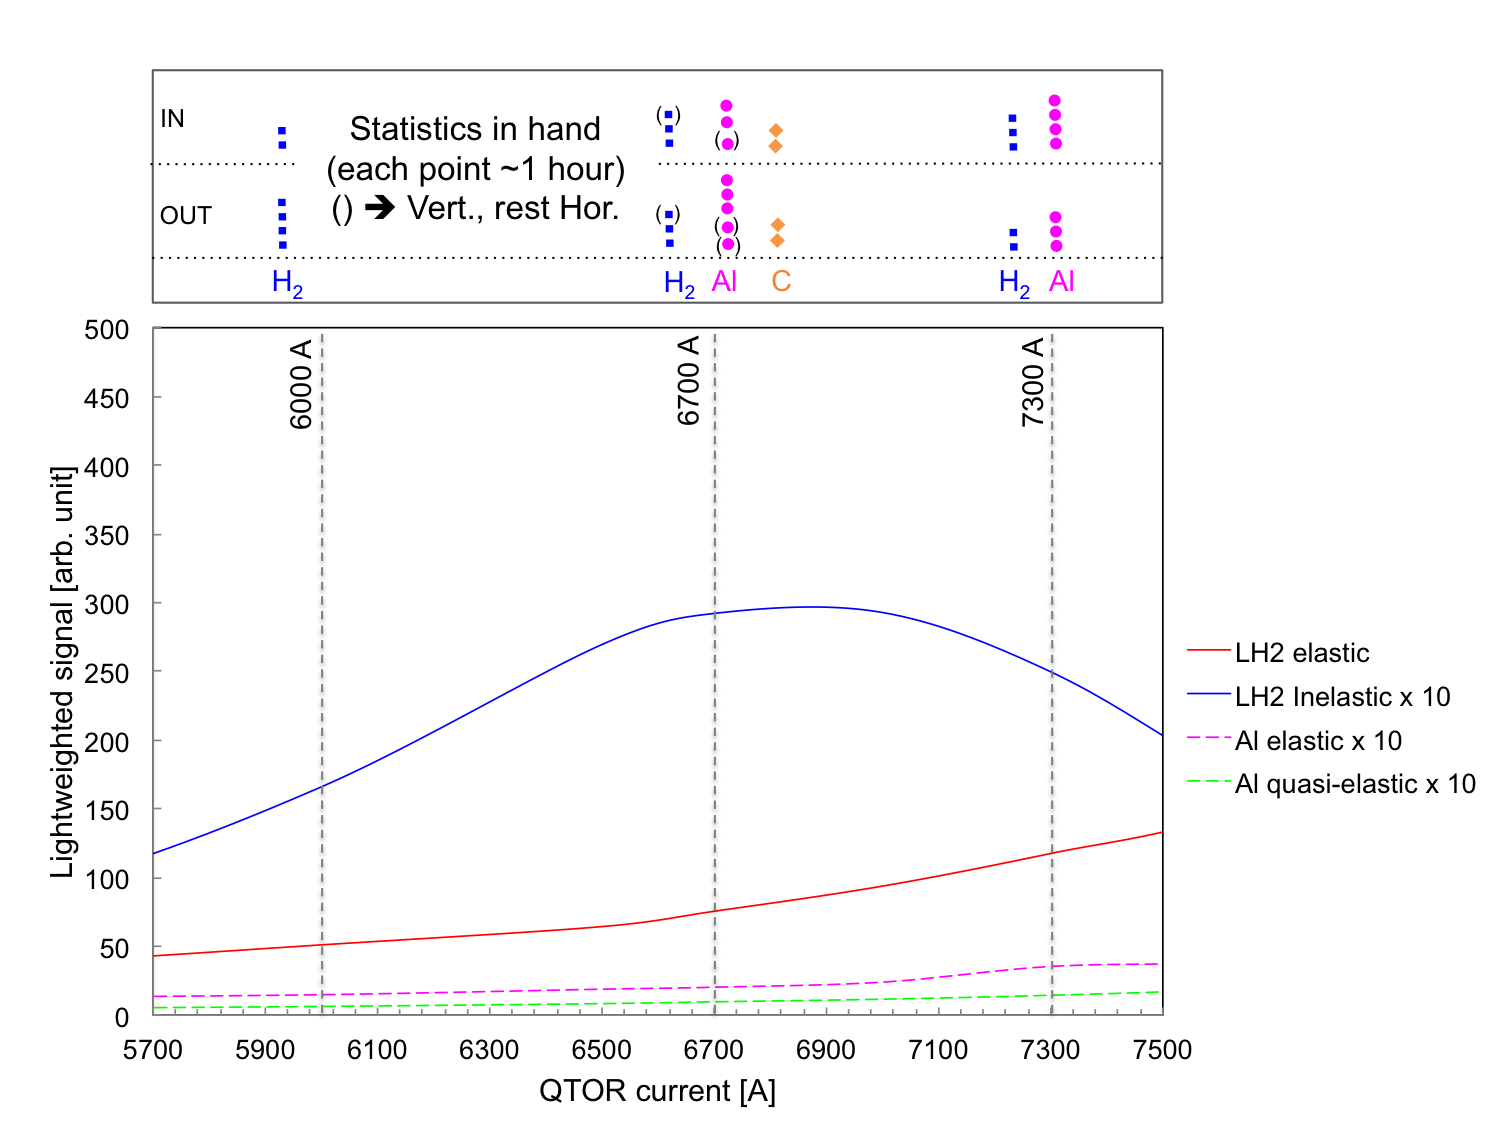
\includegraphics[width=5.0cm]{figures/transverseN2Delta}}
\hspace{-0.17em}\only<5>{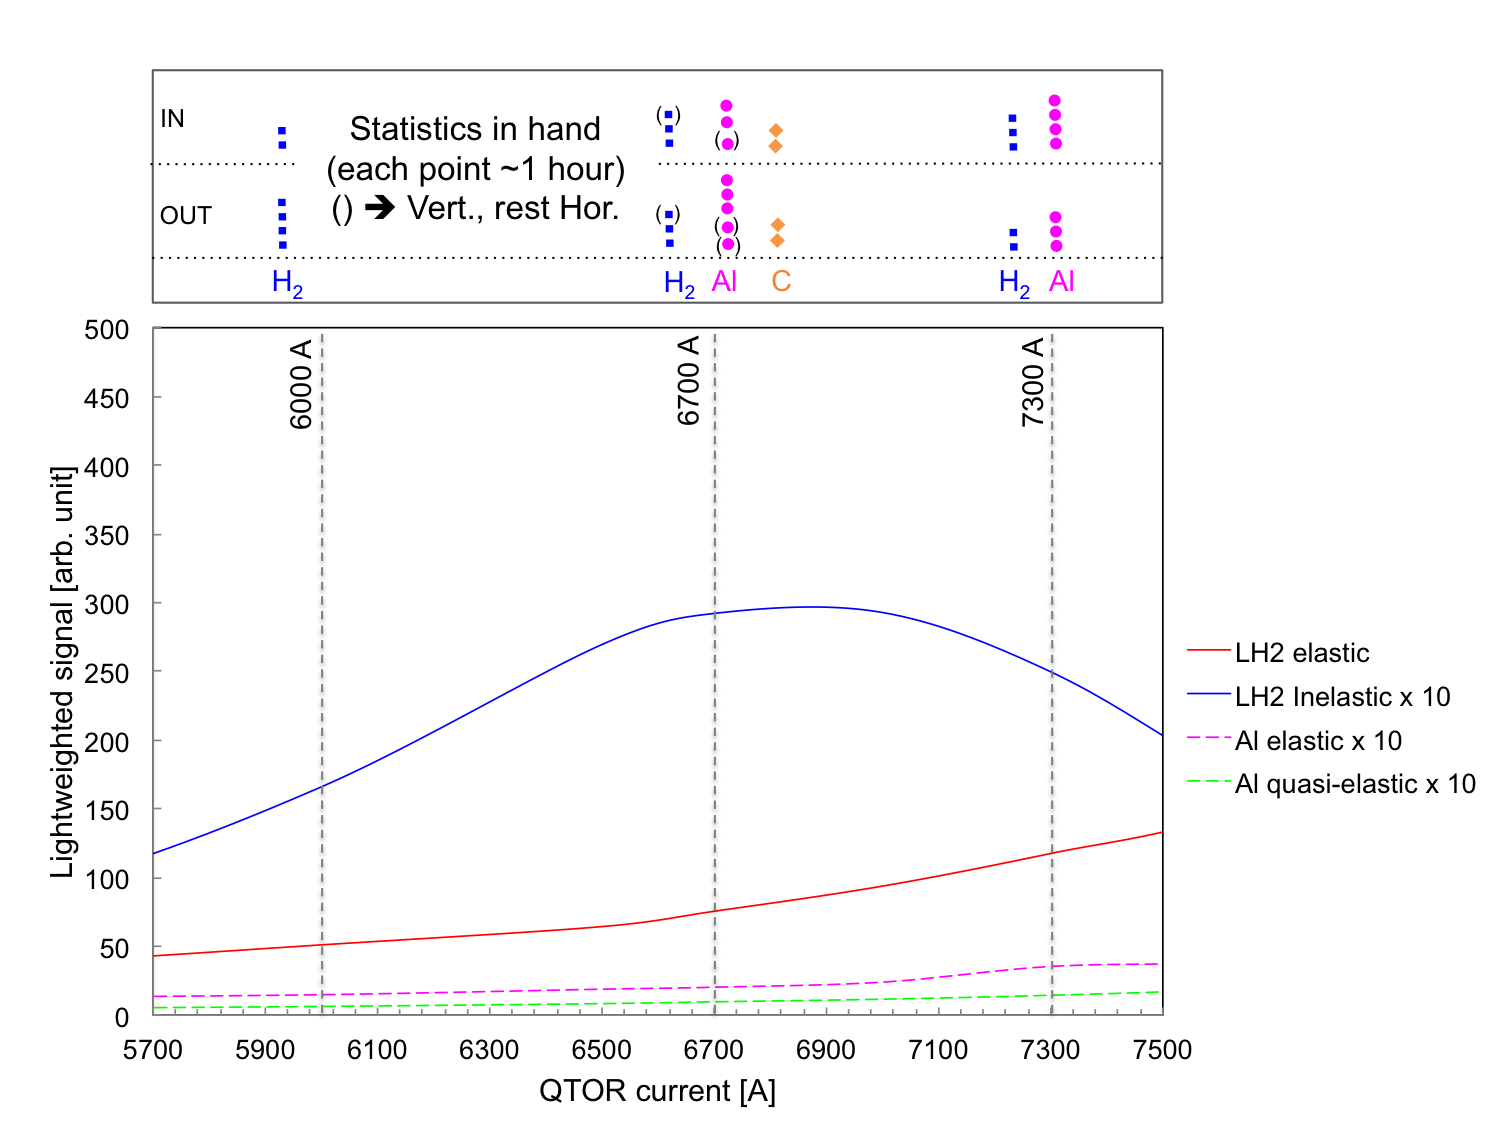
\includegraphics[width=5.0cm]{figures/transverseN2Delta}}

\only<2-5>{\mbox{\structure{Figure:} something}}

%\visible<2->{
%   \textbf{Some text}
%   \begin{figure}[ht]
%	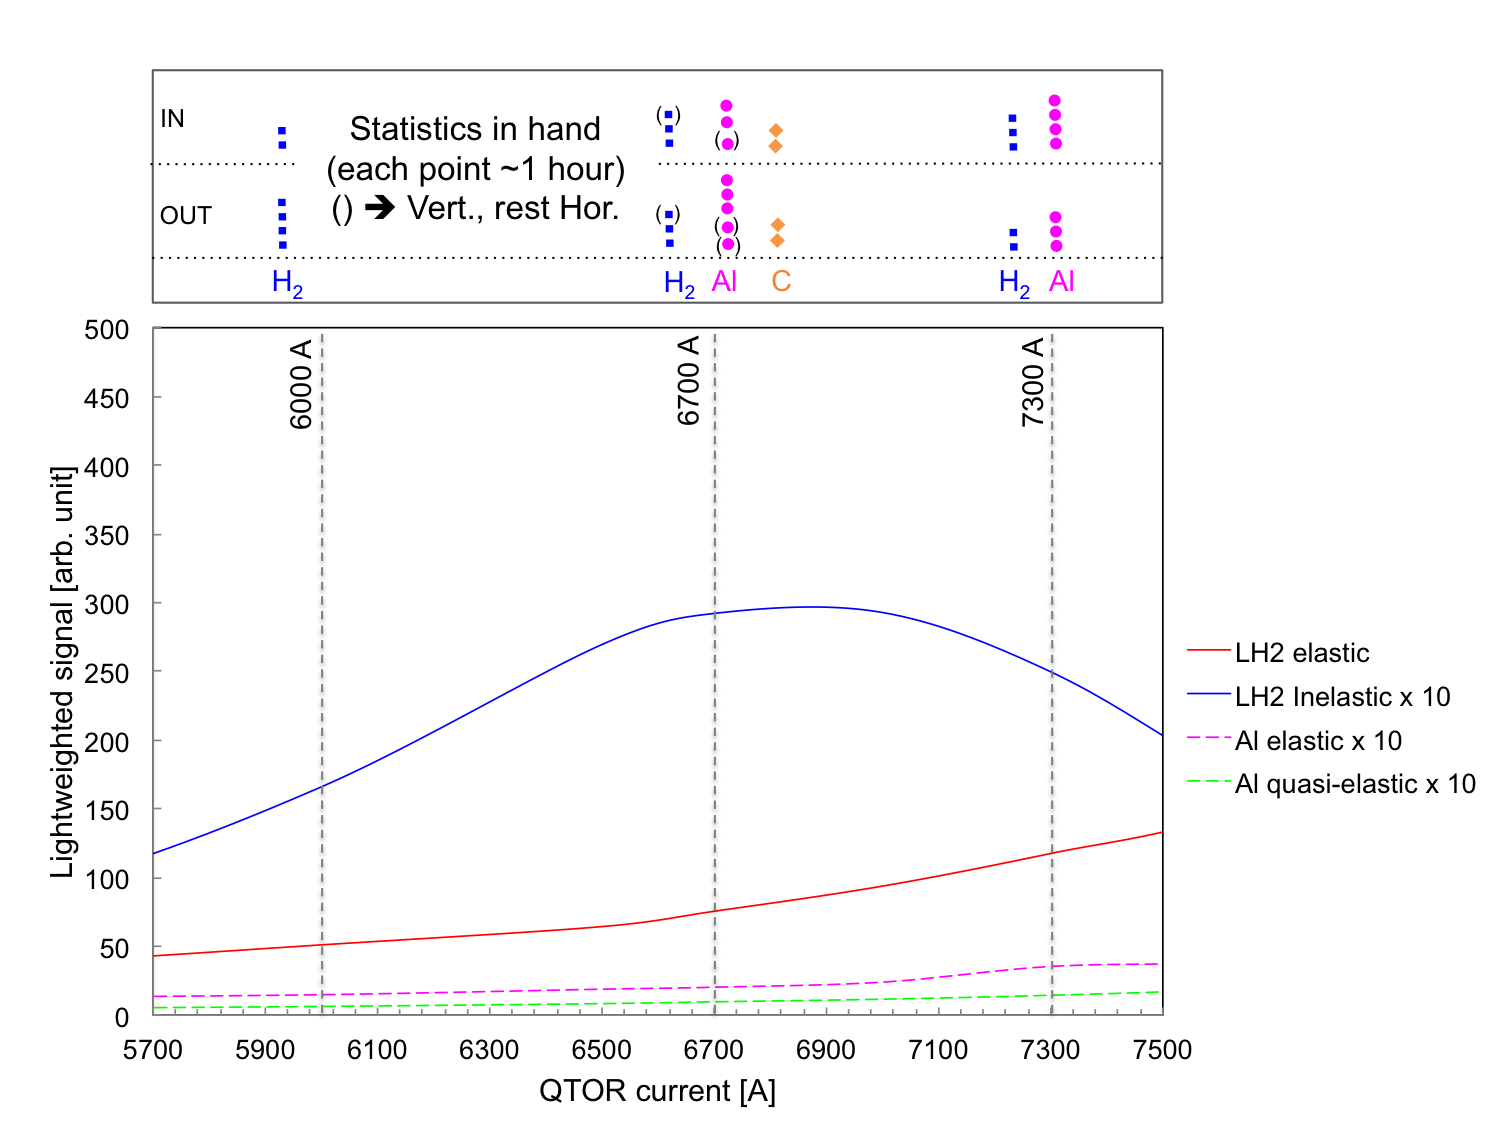
\includegraphics[width=5.0cm]{figures/transverseN2Delta}
%    \end{figure}
% }

\end{frame}



%%%%%%%%%%%%%%%%%%%%%%%%%%%%%%%%%%%%%%%%%%%%%%%%%%%%%%
%%%%%%%%%%%%%%%%%%%%%%%%%%%%%%%%%%%%%%%%%%%%%%%%%%%%%%
\section{\scshape Methodology}
\subsection{Frame 6}

\begin{frame}{Frame 6}

\fontsize{6pt}{7.2}\selectfont

Some basic formalism about qweak.

\begin{equation} \label{equ:qweak1}
A_{ep} = \left[ \frac{-G_{F}Q^{2}}{4 \sqrt{2}\pi\alpha} \right] \left[ \frac{\varepsilon G_{E}^{\gamma}G_{E}^{Z} + \tau G_{M}^{\gamma}G_{M}^{Z} - (1-4\sin^{2}\theta_{W})\varepsilon^{\prime}G_{M}^{\gamma}G_{A}^{Z} } { \varepsilon(G_{E}^{\gamma})^{2} + \tau(G_{M}^{\gamma})^{2} } \right]
\end{equation}

\begin{equation} \label{equ:qweak2}
\varepsilon = \frac{1}{1 + 2(1+\tau)\tan^{2}\frac{\theta}{2}}, \varepsilon^{\prime} = \sqrt{\tau(1+\tau)(1 - \varepsilon^{2})}, \tau = \frac{Q^{2}}{4M}
\end{equation}

\fontsize{10pt}{7.2}\selectfont

As $\theta$ $\rightarrow$ 0, $\varepsilon$ $\rightarrow$ 1, and $\tau$ $\ll$ 1


\end{frame}

\begin{frame}{Frame 7}

\begin{equation} \label{equ:qweak3}
A_{ep} = \left[ \frac{-G_{F}Q^{2}}{4 \sqrt{2}\pi\alpha} \right] \left[ Q_{W}^{p} + B(Q^{2}, \theta) \right] = A_{0} \left[ Q_{W}^{p} + B(Q^{2}, \theta) \right]
\end{equation}

\begin{equation} \label{equ:qweak5}
A_{ep} = \left[ \frac{-G_{F}Q^{2}}{4 \sqrt{2}\pi\alpha} \right] \left[ Q_{W}^{p} + Q^{2}B(Q^{2}, \theta) \right] = A_{0} \left[ Q_{W}^{p} + Q^{2}B(Q^{2}, \theta) \right]
\end{equation}

\begin{equation} \label{equ:qweak4}
\begin{split}
A_{ep} = A_{0} \left[ Q_{W}^{p} + B(Q^{2}, \theta) \right]\\
A_{0} = \frac{-G_{F}Q^{2}}{4 \sqrt{2}\pi\alpha}
\end{split}
\end{equation}


\begin{equation} \label{equ:qweak6}
\begin{split}
\sigma \approx \vert M_{EM} + M_{weak} \vert^{2} \\
\sigma \approx \vert M_{EM} \vert^{2} + 2M_{EM}^{*}M_{weak} + \vert M_{weak} \vert^{2}  \\
\sigma \approx \vert M_{EM} \vert^{2} 
\end{split}
\end{equation}

\end{frame}

%\begin{singlespace}
%\begin{table}
%\begin{center}
%  \begin{tabular}{| c | c | c  c  c |}
%    \hline
%    Particle & EM Charge &  & Weak Charge &  \\ \hline
%    u-quark & +$\frac{2}{3}$ & -2$C_{1u}$ & = $1 - \frac{8}{3}\sin^{2}\theta_{W}$ & $\approx$ +$\frac{1}{3}$ \\
%    d-quark & -$\frac{1}{3}$ & -2$C_{1d}$ & = $-1 + \frac{4}{3}\sin^{2}\theta_{W}$ & $\approx$ -$\frac{1}{3}$ \\
%    proton (uud) & 1 & $Q_{W}^{p}$ = -2(2$C_{1u}$+$C_{1d}$) & = $1 - 4\sin^{2}\theta_{W}$ & $\approx$ 0.07 \\
%    neutron (udd) & 0 & $Q_{W}^{n}$ = -2($C_{1u}$+2$C_{1d}$) & & $\approx$ -1 \\
%    \hline
%  	\end{tabular}
%  	\caption[Dead time calculation for beam modulation]{Dead time calculation for beam modulation}
%  \label{tQweak11}
%\end{center}
%\end{table}
%\end{singlespace}


\begin{frame}{Frame 8}

\begin{equation} \label{equ:qweak6}
\begin{split}
A_{ep} = \frac{ \sigma_{+} - \sigma_{-} }{ \sigma_{+} + \sigma_{-} } \approx \frac{2 \Re \vert M_{EM}\cdot M_{weak} \vert }{\vert M_{EM} \vert^{2} }
\end{split}
\end{equation}

\pause

\begin{equation} \label{equ:qweak61}
A_{msr} = \frac{ Y_{+} - Y_{-} }{ Y_{+} + Y_{-} }
\end{equation}

%\pausecolors{red}{black}{highlighted}
 
\begin{equation} \label{equ:qweak62}
A_{ep} = \frac{ A_{msr} -  \displaystyle\sum_{i} A^{i}_{false} }{ P }
\end{equation}

\begin{equation} \label{equ:qweak64}
\begin{split}
A_{ep} = \frac{ \sigma_{+} - \sigma_{-} }{ \sigma_{+} + \sigma_{-} } \approx \frac{\vert M_{weak}^{PV} \vert }{\vert M_{EM} \vert }
\end{split}
\end{equation}

\begin{equation} \label{equ:qweak63}
\begin{split}
A_{ep} \approx \frac{2 \Re \vert M_{EM}\cdot M_{weak} \vert }{\vert M_{EM} \vert^{2} } = \frac{ \sigma_{+} - \sigma_{-} }{ \sigma_{+} + \sigma_{-} }
\end{split}
\end{equation}



Where $\sigma_{+}$($\sigma_{-}$) is the positive (negative) helicity correlated electron-proton scattering cross sections. $M_{weak}$ and $M_{EM}$ are the parity violating and parity conserving electromagnetic scattering amplitudes, respectively


\begin{equation} \label{equ:qweak7}
Q_{W}(Z,N) = -2[C_{1u}(2Z+N) +  C_{1d}(Z+2N) ]
\end{equation}

\end{frame}



\begin{frame}{Frame 9}

\textcolor{red}{
\begin{equation} \label{equ:eqPhysicsAsymmetry211}
A_{N} = R_{total} \left[ \frac{\frac{A_{M}^{in}}{P} - \displaystyle\sum_{i=1}^{4} A_{bi}f_{bi} }{1 - \displaystyle\sum_{i=1}^{4}f_{bi}} \right] 
\end{equation}
}


\begin{equation} \label{equ:eqPhysicsAsymmetry2}
A_{ep} = R_{total} \left[ \frac{\frac{A_{msr}}{P} - \displaystyle\sum_{i=1}^{4} A_{i}f_{i} }{1 - \displaystyle\sum_{i=1}^{4}f_{i}} \right] 
\end{equation}

\pause

\begin{equation} \label{equ:eqPhysicsAsymmetry3}
R_{total} = R_{RC}R_{Det}R_{Bin}R_{Q^{2}}
\end{equation}

\begin{equation} \label{equ:eqPhysicsAsymmetry4}
A_{msr} = A_{raw} + A_{T} + A_{L} + A_{reg}
\end{equation}


\begin{equation} \label{equ:eqPhysicsAsymmetry}
A_{ep} = R_{RC}R_{Det}R_{Bin} \left[ \frac{\frac{A_{msr}}{P} - A_{b1}f_{b1} - A_{b2}f_{b2} - A_{b3}f_{b3} - A_{b4}f_{b4} }{1 - f_{b1} - f_{b2} - f_{b3} - f_{b4}} \right] 
\end{equation}

%\begin{equation} \label{equ:eqPhysicsAsymmetry}
%A^{in}_{PHYS} = R_{RC}R_{Det} \left[ \frac{\frac{A^{in}_{M}}{P} - R^{A}_{b1} A_{b1}f_{b1} - A_{b2}f_{b2} - A_{b3}f_{b3} - R^{A}_{b4} A_{b4}f_{b4} }{1 - f_{b1} - f_{b2} - f_{b3} - f_{b4}} \right] 
%\end{equation}

\begin{equation} \label{equ:eqdPhysicsAsymmetryAmsr}
(dA^{in}_{PHYS})_{A_{M}^{in}} = R_{RC}R_{Det} \frac{dA^{in}_{M}}{P} \left[ \frac{ 1 }{1 - f_{b1} - f_{b2} - f_{b3} - f_{b4}} \right] 
\end{equation}

\begin{equation} \label{equ:eqdPhysicsAsymmetryP}
(dA^{in}_{PHYS})_{P} = R_{RC}R_{Det} \frac{A^{in}_{M}}{P} \frac{dP}{P} \left[ \frac{ 1 }{1 - f_{b1} - f_{b2} - f_{b3} - f_{b4}} \right] 
\end{equation}

\begin{equation} \label{equ:eqdPhysicsAsymmetryAb1}
(dA^{in}_{PHYS})_{A_{b1}} = R_{RC}R_{Det} \left[ \frac{ -dA_{b1}f_{b1} }{1 - f_{b1} - f_{b2} - f_{b3} - f_{b4}} \right] 
\end{equation}

\begin{equation} \label{equ:eqdPhysicsAsymmetryAb2}
(dA^{in}_{PHYS})_{A_{b2}} = R_{RC}R_{Det} \left[ \frac{ -dA_{b2}f_{b2} }{1 - f_{b1} - f_{b2} - f_{b3} - f_{b4}} \right] 
\end{equation}

\begin{equation} \label{equ:eqdPhysicsAsymmetryAb3}
(dA^{in}_{PHYS})_{A_{b3}} = R_{RC}R_{Det} \left[ \frac{ -dA_{b3}f_{b3} }{1 - f_{b1} - f_{b2} - f_{b3} - f_{b4}} \right] 
\end{equation}

\begin{equation} \label{equ:eqdPhysicsAsymmetryAb4}
(dA^{in}_{PHYS})_{A_{b4}} = R_{RC}R_{Det} \left[ \frac{ -dA_{b4}f_{b4} }{1 - f_{b1} - f_{b2} - f_{b3} - f_{b4}} \right] 
\end{equation}

\end{frame}

\begin{frame}{Frame 10}

\begin{equation} \label{equ:eqdPhysicsAsymmetryfb1}
(dA^{in}_{PHYS})_{f_{b1}} = R_{RC}R_{Det} df_{b1} \left[ \frac{ \frac{A^{in}_{M}}{P} - A_{b1}(1 - f_{b2} - f_{b3} - f_{b4}) - A_{b2}f_{b2} - A_{b3}f_{b3} - A_{b4}f_{b4} }{ (1 - f_{b1} - f_{b2} - f_{b3} - f_{b4})^{2} } \right] 
\end{equation}

\begin{equation} \label{equ:eqdPhysicsAsymmetryfb2}
(dA^{in}_{PHYS})_{f_{b2}} = R_{RC}R_{Det} df_{b2} \left[ \frac{ \frac{A^{in}_{M}}{P} - A_{b1}f_{b1} - A_{b2}(1 - f_{b1} - f_{b3} - f_{b4}) - A_{b3}f_{b3} - A_{b4}f_{b4} }{ (1 - f_{b1} - f_{b2} - f_{b3} - f_{b4})^{2} } \right] 
\end{equation}

\begin{equation} \label{equ:eqdPhysicsAsymmetryfb3}
(dA^{in}_{PHYS})_{f_{b3}} = R_{RC}R_{Det} df_{b3} \left[ \frac{ \frac{A^{in}_{M}}{P} - A_{b1}f_{b1} - A_{b2}f_{b2} - A_{b3}(1 - f_{b1} - f_{b2} - f_{b4}) - A_{b4}f_{b4} }{ (1 - f_{b1} - f_{b2} - f_{b3} - f_{b4})^{2} } \right] 
\end{equation}

\begin{equation} \label{equ:eqdPhysicsAsymmetryfb4}
(dA^{in}_{PHYS})_{f_{b4}} = R_{RC}R_{Det} df_{b4} \left[ \frac{ \frac{A^{in}_{M}}{P} - A_{b1}f_{b1} - A_{b2}f_{b2} - A_{b3}f_{b3} - A_{b4}(1 - f_{b1} - f_{b2} - f_{b3}) }{ (1 - f_{b1} - f_{b2} - f_{b3} - f_{b4})^{2} } \right] 
\end{equation}

\end{frame}

%\begin{frame}{Frame 1}

%%%%%%%%%%%%%%%%%%%%%%%%%%%%%%%%%%%%%%%%%%%%%%%%%%%%%%%
%%%%%%%%%%%%%%%%%%%%%%%%%%%%%%%%%%%%%%%%%%%%%%%%%%%%%%%
%\subsection{frame 5}
%\begin{frame}{frame 5}
%
%
%\def\boundb{(-2,2) rectangle (4,-2)}
%\foreach \xb in {0,0.1,...,2.1}{
%    \def\setA{(0,0) circle (1)}
%    \def\setB{(\xb,0) circle (1)}
%
%    \begin{tikzpicture}
%    \draw \boundb;
%    % intersection
%    \begin{scope}
%    \clip \setA;
%    \fill[black!20] \setB;
%    \end{scope}
%     \begin{scope}[even odd rule]% first circle without the second
%        \clip \setB \boundb;
%        \fill[red!20] \setA;
%     \end{scope}
%    \begin{scope}[even odd rule]% first circle without the second
%        \clip \setA \boundb;
%        \fill[blue!20] \setB;
%     \end{scope}
%    \draw \setA;
%    \draw \setB;
%    \node at (-1,0) [left] {$A$};
%    \node at (\xb+1,0) [right] {$B$};
%
%    \node at (4,2) [below left] {$A\cap B$};
%
%    \end{tikzpicture}
%} 
%
%\end{frame}
%%%%%%%%%%%%%%%%%%%%%%%%%%%%%%%%%%%%%%%%%%%%%%%%%%%%%%
%%%%%%%%%%%%%%%%%%%%%%%%%%%%%%%%%%%%%%%%%%%%%%%%%%%%%%
\section{\scshape Methodology}
\subsection{frame 43}

% For every picture that defines or uses external nodes, you'll have to
% apply the 'remember picture' style. To avoid some typing, we'll apply
% the style to all pictures.
\tikzstyle{every picture}+=[remember picture]

% By default all math in TikZ nodes are set in inline mode. Change this to
% displaystyle so that we don't get small fractions.
\everymath{\displaystyle}

\begin{frame}
\frametitle{Rigid body dynamics}

\tikzstyle{na} = [baseline=-.5ex]

\begin{itemize}[<+-| alert@+>]
    \item Coriolis acceleration
        \tikz[na] \node[coordinate] (n1) {};
\end{itemize}

% Below we mix an ordinary equation with TikZ nodes. Note that we have to
% adjust the baseline of the nodes to get proper alignment with the rest of
% the equation.
\begin{equation*}
\vec{a}_p = \vec{a}_o+\frac{{}^bd^2}{dt^2}\vec{r} +
        \tikz[baseline]{
            \node[fill=blue!20,anchor=base] (t1)
            {$ 2\vec{\omega}_{ib}\times\frac{{}^bd}{dt}\vec{r}$};
        } +
        \tikz[baseline]{
            \node[fill=red!20, ellipse,anchor=base] (t2)
            {$\vec{\alpha}_{ib}\times\vec{r}$};
        } +
        \tikz[baseline]{
            \node[fill=green!20,anchor=base] (t3)
            {$\vec{\omega}_{ib}\times(\vec{\omega}_{ib}\times\vec{r})$};
        }
\end{equation*}

\begin{itemize}[<+-| alert@+>]
    \item Transversal acceleration
        \tikz[na]\node [coordinate] (n2) {};
    \item Centripetal acceleration
        \tikz[na]\node [coordinate] (n3) {};
\end{itemize}

% Now it's time to draw some edges between the global nodes. Note that we
% have to apply the 'overlay' style.
\begin{tikzpicture}[overlay]
        \path[->]<1-> (n1) edge [bend left] (t1);
        \path[->]<2-> (n2) edge [bend right] (t2);
        \path[->]<3-> (n3) edge [out=0, in=-90] (t3);
\end{tikzpicture}

%A_{ep} = R_{total} \left[  \frac{A_{M}/P - \displaystyle\sum_{i=1}^{4} f_{i}A_{i} }{1- \displaystyle\sum_{i=1}^{4} f_{i} } \right] 
\end{frame}



%%%%%%%%%%%%%%%%%%%%%%%%%%%%%%%%%%%%%%%%%%%%%%%%%%%%%%
%%%%%%%%%%%%%%%%%%%%%%%%%%%%%%%%%%%%%%%%%%%%%%%%%%%%%%

\end{document}